\begin{refsection}

\section*{Abstract}
% FRAMEWORK
In this paper a unified probabilistic framework for solving inverse problems in the presence of epistemic and aleatory uncertainty is presented.
% EXPERIMENTAL SITUATIONS
The aim is to establish a flexible theory that facilitates Bayesian data analysis in experimental scenarios as they are commonly met in engineering practice.
% PROBLEM STATEMENT
Problems are addressed where learning about unobservable inputs of a forward model,
e.g.\ reducing the epistemic uncertainty of fixed yet unknown parameters and/or quantifying the aleatory uncertainty of variable inputs,
is based on processing response measurements.
% MAIN SOURCES & % FINAL FRAMEWORK
Approaches to Bayesian inversion, hierarchical modeling and uncertainty quantification are combined into a generic framework
that eventually allows to interpret and accomplish this task as multilevel model calibration.
% EQUIVALENT FORMULATIONS
A joint problem formulation, where quantities that are not of particular interest are marginalized out from a joint posterior distribution,
or an intrinsically marginal formulation, which is based on an integrated likelihood function,
can be chosen according to the inferential objective and computational convenience.
% PROBABILISTIC INVERSION
Fully Bayesian probabilistic inversion, i.e.\ the inference the variability of unobservable model inputs across a number of experiments, is derived as a special case of multilevel inversion.
% BORROWING STRENGTH
Borrowing strength, i.e.\ the optimal estimation of experiment-specific unknown forward model inputs, is introduced as a means for combining information in inverse problems.
% (IM)``PERFECT'' DATA
Two related statistical models for situations involving finite or zero model/measurement error are devised.
% COMPUTATIONAL OBSTACLES
Multilevel-specific obstacles to Bayesian posterior computation via Markov chain Monte Carlo are discussed.
% NUMERICAL DEMONSTRATION
The inferential machinery of Bayesian multilevel model calibration and its underlying flow of information are studied on the basis of a system from the domain of civil engineering.
A population of identically manufactured structural elements serves as an exemplary system for examining different experimental settings from the standpoint of uncertainty quantification and reduction.
% SPECIAL CASES
In a series of tests the material variability throughout the ensemble of specimens, the entirety of specimen-specific material properties
and the measurement error level are inferred under various uncertainties in the problem setup.

\section{Introduction}
%%%%%%%%%%%%%%%%
% INTRODUCTION %
%%%%%%%%%%%%%%%%
Main characteristics and challenges of inverse problems in engineering sciences subsume the following issues.
% FORWARD MODELING
Firstly, the ever-growing complexity of physical modeling increases the computational expense of deterministic forward simulations.
% UNCERTAINTY MODELING
Secondly, uncertainty is omnipresent and calls for an adequate mathematical formalism of representation and management.
% SCARCE DATA
Thirdly, since data are commonly scarce or prohibitively expensive to acquire, the available information has to be carefully handled.
% GENERIC PROBLEM
An abstract inverse problem statement thus reads as follows.
By analyzing a limited amount of data the endeavor is to optimally learn about unknown forward model inputs that are subject to epistemic uncertainty and aleatory variability.
% (HYPER)PARAMETERS
This includes deducing fixed albeit unknown forward model parameters as well as hyperparameters that determine the distribution of variable model inputs.
% NO PREVIOUS SOLUTION
Such a universal formulation describes a class of inverse problems that has hardly been satisfactorily solved yet.
% MOTIVATION
Our goal is therefore to develop a rigorous and extensive framework for formulating and solving such inverse problems in support of data analysis for engineering systems.
% RESEARCH FOCUS
The focus of this research is on experimental situations as they are typically encountered in this field.
We emphasize aspects of uncertainty quantification and information accumulation.
% FRAMEWORK
In order to establish a sound conceptional and computational basis for solving those problems one has to complement ideas and techniques that have been developed in different academic disciplines and scientific communities so far.
% SOURCES
This involves inverse modeling, Bayesian statistics and uncertainty quantification.
In the following we will shortly survey relevant theories and practices.
%%%%%%%%%%%%%%%%%%%%%%%%%
\par % INVERSE PROBLEMS %
%%%%%%%%%%%%%%%%%%%%%%%%%
In the first place we rely on the Bayesian approach to \textit{classical inverse problems} \cite{Bayesian:Stuart2010,Bayesian:Allmaras2013}.
% PROBLEM CHARACTERISTICS
When a physical theory or a computational solver relates physical parameters to measurable quantities, i.e.\ the \textit{forward model},
classical inversion is the process of reasoning or inferring unknown yet physically fixed model parameters from recorded data \cite{Inversion:Tarantola2005,Inversion:Kaipio2005}.
% BAYESIAN INFERENCE
Bayesian inference establishes a convenient probabilistic framework to accomplish this conventional type of parameter estimation and data assimilation.
% ENGINEERING APPLICATIONS
At least since the advent of the personal computer it is nowadays widely used in engineering applications \cite{Bayesian:Hadidi2008,Bayesian:Beck2010}.
% HIERARCHICAL INVERSION
The stochastic paradigm provides a natural mechanism for the regularization of ill-posed problems, however, it requires the specification of a prior and a noise model.
\textit{Hierarchical inversion} is an extension of the classical framework that allows to set parameters of the prior and the noise model in a data-informed manner \cite{Multilevel:Malinverno2004,Inversion:Wang2005:b}.
% CHARACTERISTICS & DEFICIENCIES
While epistemic uncertainty is naturally incorporated, a shortcoming of these types of parameter estimation is that they do not account for aleatory variability.
%%%%%%%%%%%%%%%%%%%%%%%%%%%%
\par % HIERARCHICAL MODELS %
%%%%%%%%%%%%%%%%%%%%%%%%%%%%
In the second place \textit{hierarchical statistical models} serve as the main tool for the analysis of complex systems.
Those are systems that are hierarchically organized at multiple nested layers.
% RANDOM EFFECTS
Prominent instances include \textit{random} and \textit{mixed effects models} \cite{Multilevel:Wu2010}.
% HISTORICALLY SPEAKING
Historically those models were developed in social and biological sciences e.g.\ for purposes of educational research
\cite{Multilevel:Raudenbusch1988,Multilevel:Seltzer1996} and pharmacokinetics/dynamics \cite{Multilevel:Wakefield1996,Multilevel:Banks2004}.
% RECENT REVIEWS
Some recent reviews about the methods that were developed in these fields can be found in \cite{Multilevel:Davidian2003,Multilevel:Banks2012}.
% FREQUENTISM VS. BAYESIANISM
Hierarchical modeling can be viewed from a more frequentist \cite{Multilevel:Davidian1995,Multilevel:Banks2014} or a more Bayesian perspective \cite{Multilevel:Gelman2006:a,Bayesian:Congdon2010}.
% NOWADAYS IMPORTANCE
At the present day it is mature area of research that establishes sort of an overarching theme in modern multidisciplinary statistics.
Dedicated chapters can be found in numerous standard references for Bayesian modeling and inference \cite{Bayesian:Jackman2009,Bayesian:Gelman2014:3rd}.
% CHARACTERISTICS & DEFICIENCIES
A general observation is that hierarchical models may be complex in their probabilistic architecture whereas only little forward modeling takes place.
%%%%%%%%%%%%%%%%%%%%%%%%%%%%%
\par % UNCERTAINTY MODELING %
%%%%%%%%%%%%%%%%%%%%%%%%%%%%%
In the third place we respect the uncertainty taxonomy that is prevalent in risk assessment and decision making.
According to this classification one distinguishes between epistemic and aleatory uncertainty \cite{Uncertainty:Faber2005,Uncertainty:Kiureghian2009}.
% EPISTEMIC UNCERTAINTY
On one side, \textit{epistemic uncertainty} refers to the ignorance or lack of knowledge of the observer and analyst.
By taking further evidence this type of uncertainty is reducible in principle.
% ALEATORY VARIABILITY
On the contrary, \textit{aleatory uncertainty} or \textit{variability} refers to a trait of the system under consideration.
It is a structural randomness of irreducible character.
% UNCERTAINTY REPRESENTATION
Uncertainties can be accounted for in distinct mathematical frameworks and especially the representation of ignorance is the subject matter of ongoing debates \cite{Uncertainty:Helton2004,Uncertainty:Helton2011}.
% BAYESIAN NETWORKS (BPN)
Graphical statistical models such as \textit{Bayesian probability networks} establish a powerful and widespread tool of uncertainty characterization \cite{Bayesian:Koski2009,Bayesian:Kjaerulff2013}.
In risk-based decision making Bayesian belief networks have been adopted for their strength and flexibility in uncertainty modeling \cite{Bayesian:Bayraktarli2011:a,Bayesian:Deublein2013}
and their elegant mechanisms of information aggregation \cite{Bayesian:Kelly2009,Bayesian:Urbina2012}.
%%%%%%%%%%%%%%%%%%%%%%%%%%%%%%%%
\par % PROBABILISTIC INVERSION %
%%%%%%%%%%%%%%%%%%%%%%%%%%%%%%%%
In the fourth place \textit{probabilistic inverse problems} constitute a challenging class of inverse problems that is of theoretical and practical relevance alike.
% INFERENCE OF VARIABILITY
While classical inversion is concerned with estimating uncertain yet physically fixed parameters in a series of experiments, i.e.\ identifying an epistemically uncertain quantity,
probabilistic inversion deals with inferring the distribution of such forward model inputs that vary throughout the experiments, i.e.\ quantifying their aleatory variability.
% LITERATURE REVIEW
Previously established approaches to this interesting type of problems with \textit{latent/hidden variable} structure subsume various approximate solutions.
% LIKELIHOOD MARGINALIZATION
A frequentist technique that is premised on the simulation of an explicitly marginalized likelihood is proposed in \cite{Multilevel:Rocquigny2009}.
% EXPECTATION-MAXIMIZATION (EM)
There are also attempts to compute approximate solutions based on variants of the expectation-maximization algorithm
within a linearized Gaussian frame \cite{Multilevel:Celeux2010} or with the aid of Kriging surrogates \cite{Multilevel:Barbillon2011}.
% OVERVIEW
A methodological review of this school of probabilistic inversion is found in \cite{Uncertainty:Rocquigny2012}.
% CHARACTERISTICS & DEFICIENCIES
These methods are only partly Bayesian and suffer from the deficiency of providing mere point estimates.
%%%%%%%%%%%%%%%%%%%%%%%%%
\par % BRIDGING THE GAP %
%%%%%%%%%%%%%%%%%%%%%%%%%
The potential of hierarchical models as instruments of statistical modeling and uncertainty quantification have barely been acknowledged for the purposes of inversion in a classical sense.
% HIERARCHICAL & PROBABILISTIC INVERSION
Hierarchical and probabilistic inversion are first steps towards preparing the Bayesian framework for the treatment of more realistic experimental scenarios.
These approaches do not fully exhaust the inferential machinery of hierarchical models and the probability logic of Bayesian networks, though.
% OUR CONTRIBUTION
In this contribution we thus aim at bridging that gap by developing a coherent Bayesian framework for managing uncertainties in such undertakings.
% MULTILEVEL FRAMEWORK
By drawing on the statistical theory of hierarchical models, we cast inversion under parameter uncertainty and variability as \textit{Bayesian multilevel calibration}.
% JOINT VS. MARGINAL & NUMERICAL SOLUTIONS 
This embeds a joint and a marginal problem formulation of Bayesian inference under uncertainty, both of which can be numerically solved with plain vanilla or specialized Markov chain Monte Carlo methods.
\par % ENGINEERING APPLICATIONS
This new formulation of \textit{multilevel inversion} is especially well-adapted to the challenges that engineers are frequently faced with.
% UNCERTAINTY MODELING
It naturally allows for sophisticated uncertainty modeling which comprises both epistemic and aleatory uncertainty.
The inclusion of the former is straightforward whereas the introduction of the latter is an extension to classical parameter estimation.
% BLACKBOX POV
It also promotes a pervasive ``blackbox'' point of view on the forward model.
While this is inevitable in many complex applications, it is not readily compliant with traditional hierarchical models.
% SPECIAL CASES & EXTENSIONS
Previously established strategies of enhanced uncertainty quantification, e.g.\ hierarchical and probabilistic inversion, emerge as special cases of the proposed general problem formulation.
% FULLY BAYESIAN PROBABILISTIC INVERSION
This also offers the opportunity to cope with probabilistic inversion within a fully Bayesian setting.
% NEW IDEAS
Beyond these extensions some fundamentally new possibilities are suggested.
% ``PERFECT'' DATA
Based on the probabilistic calculus of multilevel models, we develop a novel formulation of multilevel inversion in the zero-noise and ``perfect'' data limit.
% BORROWING STRENGTH
The statistical effect of ``borrowing strength'' or ``optimal combination of information'' is transferred and applied to inverse problems.
%%%%%%%%%%%%%%%%
\par % OUTLINE %
%%%%%%%%%%%%%%%%
The article is organized as follows.
In \cref{sec:PEM:Multilevel} we will elaborate a general Bayesian framework for the treatment of uncertainty and variability in inverse problems.
This is followed by a discussion about Bayesian inference in the context of multilevel inversion in \cref{sec:PEM:Inference}.
Thereafter \cref{sec:PEM:PerfectData} will provide an extension of the framework that will allow for handling ``perfect'' data.
Probabilistic inversion and borrowing strength will be placed in context in \cref{sec:PEM:ProbInv,sec:PEM:CombInf}, respectively.
Dedicated Bayesian computations based on Markov chain Monte Carlo are reviewed in \cref{sec:PEM:Computations}.
Lastly in \cref{sec:PEM:CaseStudies} we will conduct a selection of numerical case studies, where by considering various experimental situations and uncertainty setups
the very potential and the computational challenges of the devised modeling paradigm will become transparent.

\section{Bayesian multilevel modeling} \label{sec:PEM:Multilevel}
%%%%%%%%%%%%%%%%%%%%%%%%%%%%%%%%
% BAYESIAN MULTILEVEL MODELING %
%%%%%%%%%%%%%%%%%%%%%%%%%%%%%%%%
Due to the lack of a unified terminology, we define a \textit{hierarchical} or \textit{multilevel model} as
``an overall system model that is hierarchically composed of deterministic and stochastic submodels''.
% SECTION OUTLINE
Important types of submodels comprise physical models of the deterministic system components (\cref{sec:PEM:Multilevel:ForwardModel}),
prior descriptions of parameter uncertainty and variability (\cref{sec:PEM:Multilevel:Uncertainty})
and residual representations of forward model prediction errors (\cref{sec:PEM:Multilevel:Residual}).
% GENERIC MODEL
From these submodels we will assemble a generic Bayesian multilevel model (\cref{sec:PEM:Multilevel:Overall}).
This will represent the overall system under consideration including its deterministic and probabilistic aspects.

\subsection{Forward model: Deterministic subsystem} \label{sec:PEM:Multilevel:ForwardModel}
% FORWARD MODEL: PHYSICS
A so-called \textit{forward model} is a mathematical representation of the physical system or phenomenon under investigation.
More formally the forward model is a function
\begin{equation} \label{eq:PEM:Multilevel:ForwardModel}
  \begin{aligned}
    \mathcal{M} \colon \mathcal{D}_{\bm{m}} \times \mathcal{D}_{\bm{x}} \times \mathcal{D}_{\bm{\zeta}} \times \mathcal{D}_{\bm{d}} &\rightarrow \mathcal{D}_{\perfect{\bm{y}}}\\
    (\bm{m},\bm{x},\bm{\zeta},\bm{d}) &\mapsto \perfect{\bm{y}} = \mathcal{M}(\bm{m},\bm{x},\bm{\zeta},\bm{d}),
  \end{aligned}
\end{equation}
that maps inputs \((\bm{m},\bm{x},\bm{\zeta},\bm{d}) \in \mathcal{D}_{\bm{m}} \times \mathcal{D}_{\bm{x}} \times \mathcal{D}_{\bm{\zeta}} \times \mathcal{D}_{\bm{d}}\)
from its domain to outputs \(\perfect{\bm{y}} \in \mathcal{D}_{\perfect{\bm{y}}}\) from its codomain.
% PARAMETERS / PREDICTIONS
Forward model arguments \((\bm{m},\bm{x},\bm{\zeta},\bm{d})\) constitute physical parameters, while its responses \(\perfect{\bm{y}}\) are predictions of observable quantities.
\par % FORWARD MODEL INPUTS
We distinguish between four different types of forward model inputs.
They differ in their (un)certain nature when a number of experiments is carried out.
There are fixed albeit unknown model parameters \(\bm{m} \in \mathcal{D}_{\bm{m}}\) that are subject to epistemic uncertainty,
two different types of inputs \(\bm{x} \in \mathcal{D}_{\bm{x}}\) and \(\bm{\zeta} \in \mathcal{D}_{\bm{\zeta}}\) that are subject to aleatory variability
and well-known experimental conditions \(\bm{d} \in \mathcal{D}_{\bm{d}}\).

\subsection{Prior model: Input uncertainty} \label{sec:PEM:Multilevel:Uncertainty}
%%%%%%%%%%%%%%%%%%%%%%%%%%%
% EXPERIMENTAL CONDITIONS %
%%%%%%%%%%%%%%%%%%%%%%%%%%%
Forward model inputs \(\bm{d}\) constitute perfectly known conditions that prevail during experimentation.
In line with this they are deterministic arguments of the forward model.
Experimental conditions may differ throughout the experiments, i.e.\ each of the experiments \(i=1,\ldots,n\) is conducted being subject to an experiment-specific condition \(\bm{d}_i\).
%%%%%%%%%%%%%%%%%%%%%%%%
\par % MODEL PARAMETER %
%%%%%%%%%%%%%%%%%%%%%%%%
Proper forward model parameters \(\bm{m}\) are constant throughout the experiments \(i=1,\ldots,n\), yet they have unknown values.
In Bayesian fashion the available prior or expert knowledge about the true parameter values is represented as a random variable or vector
\begin{equation} \label{eq:PEM:Multilevel:ParametricPriorM}
  \bm{M} \sim \pi_{\bm{M}} (\bm{m}).
\end{equation}
The Bayesian prior distribution \(\pi_{\bm{M}} (\bm{m})\) quantifies a subjective degree of plausibility or belief about the true parameter values \(\bm{m}\).
This is the Bayesian account for \textit{epistemic uncertainty}.
% REDUCIBILITY
The uncertainty is reducible in the sense that Bayesian data analysis gives rise to a posterior probability model.
%%%%%%%%%%%%%%%%%%%%%%%%%%
\par % KNOWN VARIABILITY %
%%%%%%%%%%%%%%%%%%%%%%%%%%
Forward model inputs \(\bm{\zeta}\) are subject to a form of variability that is well-known, e.g.\ it could be ascertained in previous experiments or due to prior considerations.
Rather than being constant throughout the experiments \(i=1,\ldots,n\), these variable inputs take on experiment-specific realizations \(\bm{\zeta}_i\), all of which are unknown.
The corresponding Bayesian prior representation is as mutually independent random variables
\begin{equation} \label{eq:PEM:Multilevel:StructuralPriorZ}
  \bm{Z}_i \sim f_{\bm{Z}}(\bm{\zeta}_i \distparam \bm{\theta}_{\bm{Z}_i}), \;\, \text{for} \;\, i=1,\ldots,n.
\end{equation}
Distributions \(f_{\bm{Z}}(\bm{\zeta}_i \distparam \bm{\theta}_{\bm{Z}_i})\) specify prior knowledge about the experiment-specific unknowns that is of structural quality.
They are prescribed by well-known hyperparameters \(\bm{\theta}_{\bm{Z}_i} \in \mathcal{D}_{\bm{\theta}_{\bm{Z}}}\), e.g.\ shape, scale and dependency parameters, that possibly differ across the experiments.
Due to stochastic independence, the appropriate joint Bayesian prior model follows as
\begin{equation} \label{eq:PEM:Multilevel:JointStructuralPriorZ}
  (\bm{Z}_1,\ldots,\bm{Z}_n) \sim \prod\limits_{i=1}^n f_{\bm{Z}}(\bm{\zeta}_i \distparam \bm{\theta}_{\bm{Z}_i}).
\end{equation}
This is a Bayesian conception of \textit{aleatory variability}, i.e.\ an uncertainty that is of structural nature.
Hereinafter this probability model will also be referred to as \textit{prescribed uncertainty}.
% IRREDUCIBILITY
It is irreducible in the sense that by Bayesian data analysis of the experiments \(i=1,\ldots,n\) ``past'' realizations \(\bm{\zeta}_i\) can be inferred in principle,
whereas the knowledge about ``future'' realizations \(\bm{\zeta}_{\further{i}}\) in further experiments \(\further{i} = n+1,\ldots,n+\further{n}\) cannot be improved.
``Future'' realizations still feature a structural uncertainty \(\bm{Z}_{\further{i}} \sim f_{\bm{Z}}(\bm{\zeta}_{\further{i}} \distparam \bm{\theta}_{\bm{Z}_{\further{i}}})\)
that is prescribed by hyperparameters \(\bm{\theta}_{\bm{Z}_{\further{i}}} \in \mathcal{D}_{\bm{\theta}_{\bm{Z}}}\).
%%%%%%%%%%%%%%%%%%%%%%%%%%%%
\par % UNKNOWN VARIABILITY %
%%%%%%%%%%%%%%%%%%%%%%%%%%%%
Another Bayesian notion of a similar type allows to account for forward model inputs \(\bm{x}\) that are subject to a sort of variability which itself is unknown.
For \(1=1,\ldots,n\) these variables take on experiment-specific realizations \(\bm{x}_i\), neither of which are known.
Bayesian prior modeling is build upon conditionally independent random variables
\begin{equation} \label{eq:PEM:Multilevel:StructuralPriorX}
  (\bm{X}_i \cond \bm{\Theta}_{\bm{X}}=\bm{\theta}_{\bm{X}}) \sim f_{\bm{X} \cond \bm{\Theta}_{\bm{X}}} (\bm{x}_i \cond \bm{\theta}_{\bm{X}}), \;\, \text{for} \;\, i=1,\ldots,n.
\end{equation}
The conditional probability distribution \(f_{\bm{X} \cond \bm{\Theta}_{\bm{X}}} (\bm{x}_i \cond \bm{\theta}_{\bm{X}})\) represents a structural kind of prior knowledge about the experiment-specific unknowns.
% HYPERPARAMETER
Its determining hyperparameters \(\bm{\theta}_{\bm{X}} \in \mathcal{D}_{\bm{\theta}_{\bm{X}}}\), e.g.\ location, dispersion and correlation parameters, themselves are fixed yet unknown.
Hence these hyperparameters are priorly modeled as a random vector
\begin{equation} \label{eq:PEM:Multilevel:ParametricPriorThetaX}
  \bm{\Theta}_{\bm{X}} \sim \pi_{\bm{\Theta}_{\bm{X}}} (\bm{\theta}_{\bm{X}}).
\end{equation}
The Bayesian prior distribution \(\pi_{\bm{\Theta}_{\bm{X}}} (\bm{\theta}_{\bm{X}})\) constitutes the subjective prior belief or available prior knowledge about the true hyperparameter values.
% PRIOR ELICITATION
In the statistical literature hyperprior elicitation is exhaustively discussed especially for variance hyperparameters \cite{Multilevel:Berger1996,Multilevel:Berger2005,Multilevel:Gelman2006:b}.
% EXCHANGEABILITY
Consequently the joint distribution of the unknowns of this prior model is given as
\begin{equation} \label{eq:PEM:Multilevel:JointStructuralPriorX}
  (\bm{X}_1,\ldots,\bm{X}_n,\bm{\Theta}_{\bm{X}}) \sim \left( \prod_{i=1}^n f_{\bm{X} \cond \bm{\Theta}_{\bm{X}}} (\bm{x}_i \cond \bm{\theta}_{\bm{X}}) \right) \pi_{\bm{\Theta}_{\bm{X}}} (\bm{\theta}_{\bm{X}}).
\end{equation}
The joint prior distribution of experiment-specific realizations follows by marginalizing \cref{eq:PEM:Multilevel:JointStructuralPriorX} over the hyperparameters \(\bm{\theta}_{\bm{X}}\).
Then one has
\begin{equation} \label{eq:PEM:Multilevel:Exchangeability}
  (\bm{X}_1,\ldots,\bm{X}_n) \sim \int\limits_{\mathcal{D}_{\bm{\theta}_{\bm{X}}}} \left( \prod\limits_{i=1}^n f_{\bm{X} \cond \bm{\Theta}_{\bm{X}}} (\bm{x}_i \cond \bm{\theta}_{\bm{X}}) \right)
  \pi_{\bm{\Theta}_{\bm{X}}} (\bm{\theta}_{\bm{X}}) \, \mathrm{d} \bm{\theta}_{\bm{X}}.
\end{equation}
This is a form of \textit{exchangeability} \cite{Multilevel:Draper1993,Multilevel:Bernardo1996} that realizes some ``similarity'' of the intermediate variables,
i.e.\ the joint distribution of the sequence \((\bm{X}_1,\ldots,\bm{X}_n)\) equals the one of \((\bm{X}_{\tau(1)},\ldots,\bm{X}_{\tau(n)})\) for any index permutation \(\tau \colon \{1,\ldots,n\} \rightarrow \{1,\ldots,n\}\).
In the present form \cref{eq:PEM:Multilevel:Exchangeability}, exchangeability establishes another Bayesian approach to aleatory variability.
% PARTIAL REDICUBILITY
Unlike the prescribed uncertainty in \cref{eq:PEM:Multilevel:JointStructuralPriorZ},  
this form of uncertainty is partially reducible in the sense that the ``fuzziness'' inherent in \cref{eq:PEM:Multilevel:Exchangeability} can be reduced by learning about \(\bm{\theta}_{\bm{X}}\) in ``past'' experiments \(i\).
``Past'' realizations \(\bm{x}_i\) can also be inferred, however, even if the hyperparameters \(\bm{\theta}_{\bm{X}}\) would be known, the realizations \(\bm{x}_{\further{i}}\) of ``future'' experiments \(\further{i}\)
would still carry the structural prior uncertainty \(\bm{X}_{\further{i}} \sim f_{\bm{X} \cond \bm{\Theta}_{\bm{X}}} (\bm{x}_{\further{i}} \cond \bm{\theta}_{\bm{X}})\).
%%%%%%%%%%%%%%%%%%%%%%
\par % SHORT SUMMARY %
%%%%%%%%%%%%%%%%%%%%%%
In short, on the one hand we have \textit{parametric priors} \(\pi_{\bm{M}} (\bm{m})\) and \(\pi_{\bm{\Theta}_{\bm{X}}} (\bm{\theta}_{\bm{X}})\)
that in \cref{eq:PEM:Multilevel:ParametricPriorM,eq:PEM:Multilevel:ParametricPriorThetaX} embody knowledge about global unknowns \(\bm{m}\) and \(\bm{\theta}_{\bm{X}}\).
On the other hand we have \textit{structural priors} \(f_{\bm{Z}}(\bm{\zeta}_i \distparam \bm{\theta}_{\bm{Z}_i})\) and
\(f_{\bm{X} \cond \bm{\Theta}_{\bm{X}}} (\bm{x}_i \cond \bm{\theta}_{\bm{X}})\) that encapsulate structural prior knowledge about the problem,
and that for \(i=1,\ldots,n\) establish the prior model of experiment-specific unknowns \(\bm{x}_i\) and \(\bm{\zeta}_i\) through \cref{eq:PEM:Multilevel:JointStructuralPriorZ,eq:PEM:Multilevel:Exchangeability}.

\subsection{Residual model: Output imperfection} \label{sec:PEM:Multilevel:Residual}
% RESIDUAL MODEL
Besides a representation of forward model input uncertainty and variability,
an integral constituent of statistical approaches to inversion is a \textit{residual representation} of forward model output discrepancy or imperfection.
Due to measurement errors, numerical approximations and general inadequacies, even if all inputs \((\bm{m},\bm{x}_i,\bm{\zeta}_i,\bm{d}_i)\) were perfectly known,
predictions \(\perfect{\bm{y}}_i = \mathcal{M}(\bm{m},\bm{x}_i,\bm{\zeta}_i,\bm{d}_i)\) are expected to deviate from real observations \(\bm{y}_i\).
These imperfections can be accounted for by a \textit{statistical data model}
\begin{equation} \label{eq:PEM:Multilevel:StatisticalDataModel}
  \bm{y}_i = \perfect{\bm{y}}_i + \bm{\varepsilon}_i = \mathcal{M}(\bm{m},\bm{x}_i,\bm{\zeta}_i,\bm{d}_i) + \bm{\varepsilon}_i,
  \;\, \text{for} \;\, i=1,\ldots,n,
\end{equation}
where residual terms \(\bm{\varepsilon}_i \in \mathcal{D}_{\bm{\varepsilon}}\) are assumed to be realizations of random variables \(\bm{E}_i \sim f_{\bm{E}}(\bm{\varepsilon}_i \distparam \bm{\Sigma}_i)\).
Commonly one employs normal distributions \(f_{\bm{E}}(\bm{\varepsilon}_i \distparam \bm{\Sigma}_i) = \mathcal{N}(\bm{\varepsilon}_i \distparam \bm{0},\bm{\Sigma}_i)\)
with mean \(\bm{0}\) and possibly experiment-specific, symmetric and positive-semidefinite covariance matrices \(\bm{\Sigma}_i\).
% RANDOM DATA
Consequently, through a change of variables whose Jacobian determinant equals one, observations are viewed as outcomes \(\bm{y}_i\) of random variables
\begin{equation} \label{eq:PEM:Multilevel:ResidualModel}
  (\bm{Y}_i \cond \bm{M} = \bm{m},\bm{X}_i = \bm{x}_i,\bm{Z}_i = \bm{\zeta}_i) \sim f_{\bm{E}} \big( \bm{y}_i-\mathcal{M}(\bm{m},\bm{x}_i,\bm{\zeta}_i,\bm{d}_i) \distparam \bm{\Sigma}_i \big),
  \;\, \text{for} \;\, i=1,\ldots,n.
\end{equation}
% CONDITIONAL STRUCTURE
For given values of the direct forward model inputs \((\bm{m},\bm{x}_i,\bm{\zeta}_i,\bm{d}_i)\),
data are viewed as random variables \((\bm{Y}_i \cond \bm{m},\bm{x}_i,\bm{\zeta}_i)\) with conditional distributions
\(f (\bm{y}_i \cond \bm{m},\bm{x}_i,\bm{\zeta}_i) = f_{\bm{E}} (\bm{y}_i-\mathcal{M}(\bm{m},\bm{x}_i,\bm{\zeta}_i,\bm{d}_i) \distparam \bm{\Sigma}_i)\).
Note that \(f (\bm{y}_i \cond \bm{m}, \allowbreak \bm{x}_i,\bm{\zeta}_i) = f (\bm{y}_i \cond \bm{m},\bm{x}_i,\bm{\zeta}_i,\bm{\theta}_{\bm{X}})\) is independent of \(\bm{\theta}_{\bm{X}}\).
\par % RESIDUAL CALIBRATION
The specification of the residual model, i.e.\ quantifying the parameters of \(\bm{\Sigma}_i\), is an essential part of calibrating the forward model and the experimental apparatus.
% PREDICTIVE ERROR CALIBRATION
In many experimental situations a model of the \textit{prediction error} is not known a priori, though.
Nevertheless, the structure of the prediction error model can be selected \cite{Bayesian:Simoen2013:a} and
its parameters can be introduced as unknown hyperparameters that undergo calibration \cite{Bayesian:Zhang2011}.
% SYSTEMATIC ERRORS & MODEL BIAS
This also includes systematic forward model deviations \cite{Bayesian:Kennedy2001,Bayesian:Arendt2012:a}.
% MODEL UNCERTAINTY
Moreover one could treat the form of the forward model \(\mathcal{M}\) itself as uncertain/random \cite{Bayesian:Droguett2008,Bayesian:Park2014}
and select the most plausible class via Bayesian model selection \cite{Bayesian:Beck2004,Bayesian:Yuen2010:b}.
% HIERARCHICAL MODELS
By adding another layer of uncertainty on top of the outlined setup and at a higher associated cost,
the aforementioned principles of assessing structural and parametric forward model uncertainty can be readily applied in multilevel models \cite{Bayesian:Draper1995}.
\par % ``PERFECT'' DATA
Based on random variable transformations, in \cref{sec:PEM:PerfectData} we will extend the framework by a model
for analyzing ``perfect'' observations \(\perfect{\bm{y}}_i = \mathcal{M}(\bm{m},\bm{x}_i,\bm{\zeta}_i,\bm{d}_i)\) in the zero-noise limit \(\lvert \bm{\varepsilon}_i \rvert \rightarrow 0\).
This mathematical formulation will explain the variability in the data exclusively by a Bayesian prior model of input variability as outlined in the preceding \cref{sec:PEM:Multilevel:Uncertainty}.

\subsection{Multilevel model: Overall system} \label{sec:PEM:Multilevel:Overall}
% (CONDITIONAL) INDEPENDENCE
We start from the premise that if not denoted or stated otherwise, random vectors and variables are (conditionally) independent,
e.g.\ the global forward model parameters \(\bm{M}\) and the hyperparameters \(\bm{\Theta}_{\bm{X}}\) are understood to be priorly independent.
Thus \(\pi(\bm{m},\bm{\theta}_{\bm{X}}) = \pi_{\bm{M}} (\bm{m}) \, \pi_{\bm{\Theta}_{\bm{X}}} (\bm{\theta}_{\bm{X}})\) applies for their joint prior distribution.
Note that this is not a necessity of the formulation, though.
% (CONDITIONAL) NOTATION
Moreover, we strictly reserve conditional notation for the stochastic dependency of random variables on outcomes of other random variables,
e.g.\ the aleatory variables \((\bm{X}_i \cond \bm{\theta}_{\bm{X}})\) are conditionally dependent on realizations \(\bm{\Theta}_{\bm{X}}=\bm{\theta}_{\bm{X}}\).
The stochastic variables \((\bm{Y}_i \cond \bm{m},\bm{x}_i,\bm{\zeta}_i)\) are conditioned on random outcomes \(\bm{M}=\bm{m}\), \(\bm{X}_i=\bm{x}_i\) and \(\bm{Z}_i=\bm{\zeta}_i\),
nonetheless they depend on deterministic quantities \(\bm{d}_i\) and \(\bm{\Sigma}_i\), too.
Similarly the aleatory variables \(\bm{Z}_i\) are dependent on \(\bm{\theta}_{\bm{Z}_i}\) in a way that is not explicitly indicated.
% BOOKKEEPING INDEX
In order to keep track of all stochastic and deterministic relations the index \(i\) serves as a bookkeeping mark.
\par % SUBMODELS
Deterministic aspects of the system are covered by the forward model \cref{eq:PEM:Multilevel:ForwardModel}.
Parametric priors in \cref{eq:PEM:Multilevel:ParametricPriorM,eq:PEM:Multilevel:ParametricPriorThetaX} and structural priors in
\cref{eq:PEM:Multilevel:StructuralPriorZ,eq:PEM:Multilevel:StructuralPriorX} represent input uncertainty and variability.
The model \cref{eq:PEM:Multilevel:ResidualModel} condenses basic assumptions regarding the prediction error.
% OVERALL MODEL
Altogether those submodels are combined into a greater model of the whole system.
The overall probability model is summarized as
\begin{subequations} \label{eq:PEM:Multilevel:Model}
  \begin{align}
    (\bm{Y}_i \cond \bm{m},\bm{x}_i,\bm{\zeta}_i) &\sim f_{\bm{E}} \big( \bm{y}_i-\mathcal{M}(\bm{m},\bm{x}_i,\bm{\zeta}_i,\bm{d}_i) \distparam \bm{\Sigma}_i \big), \label{eq:PEM:Multilevel:Model:Data}\\
    \bm{M} &\sim \pi_{\bm{M}} (\bm{m}), \label{eq:PEM:Multilevel:Model:ParametricPriorM}\\
    \bm{Z}_i &\sim f_{\bm{Z}}(\bm{\zeta}_i \distparam \bm{\theta}_{\bm{Z}_i}), \label{eq:PEM:Multilevel:Model:StructuralPriorZ}\\
    (\bm{X}_i \cond \bm{\theta}_{\bm{X}}) &\sim f_{\bm{X} \cond \bm{\Theta}_{\bm{X}}} (\bm{x}_i \cond \bm{\theta}_{\bm{X}}), \label{eq:PEM:Multilevel:Model:StructuralPriorX}\\
    \bm{\Theta}_{\bm{X}} &\sim \pi_{\bm{\Theta}_{\bm{X}}} (\bm{\theta}_{\bm{X}}). \label{eq:PEM:Multilevel:Model:ParametricPriorThetaX}
  \end{align}
\end{subequations}
% SUBJECTIVIST
Adopting a subjectivist viewpoint, this complex probability model \cref{eq:PEM:Multilevel:Model} formalizes degrees of belief of how the data have been realized in the experiments \(i=1,\ldots,n\).
% HIERARCHICAL STRUCTURE
According to our previous definition it is a generic Bayesian multilevel model.
% DAG
An intuitive representation of this multilevel model is provided by a directed acyclic graph (DAG) \cite{Bayesian:Koski2009,Bayesian:Kjaerulff2013} such as shown in \cref{fig:PEM:Multilevel:DAG}.
\begin{figure}[ht]
  \centering
  \includegraphics[height=6.5cm]{fig_PEM_DAG_Generic}
  \caption[DAG of the generic multilevel model]{DAG of the generic multilevel model.
           Vertices symbolize known (\(\vcenter{\hbox{\protect\includegraphics[height=1.2ex]{fig_Square}}}\))
           or unknown (\(\vcenter{\hbox{\protect\includegraphics[height=1.3ex]{fig_Circle}}}\)) quantities,
           while directed edges represent their deterministic (\(\vcenter{\hbox{\protect\includegraphics[height=1.0ex]{fig_Solid}}}\))
           or probabilistic (\(\vcenter{\hbox{\protect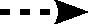
\includegraphics[height=1.0ex]{fig_Dashed}}}\)) relations.
           Global parameters \((\bm{m},\bm{\theta}_{\bm{X}})\) are subject to epistemic uncertainty,
           whereas experiment-specific realizations \((\tuple{\bm{x}_i},\tuple{\bm{\zeta}_i})\) are subject to aleatory variability.
           Known quantities comprise the data \(\tuple{\bm{y}_i}\) just as well as experiment-specific knowns
           \((\tuple{\bm{\theta}_{\bm{Z}_i}},\tuple{\bm{d}_i},\tuple{\bm{\Sigma}_i})\) located at different levels of the hierarchy.
          }
  \label{fig:PEM:Multilevel:DAG}
\end{figure}

\section{Inference in multilevel models} \label{sec:PEM:Inference}
%%%%%%%%%%%%%%%%%%%%%%%%%%%%%%%%%%
% INFERENCE IN MULTILEVEL MODELS %
%%%%%%%%%%%%%%%%%%%%%%%%%%%%%%%%%%
We will now discuss statistical inference.
In particular we will demonstrate how conditioning on the observables and marginalization out nuisance are elegant inferential tools of Bayesian multilevel inversion.
% JOINT & MARGINAL PROBLEM
A pivotal joint problem formulation will be devised.
Afterwards an intrinsically marginal problem variant will be presented in \cref{sec:PEM:Multilevel:MarginalizedFormulation}.
%%%%%%%%%%%%%%%%%%%%
\par % JOINT PRIOR %
%%%%%%%%%%%%%%%%%%%%
In the following \(\tuple{\bm{q}_i}\) denotes a sequence \(\tuple{\bm{q}_i}_{1 \leq i \leq n} = (\bm{q}_1,\bm{q}_2,\ldots,\bm{q}_n)\).
Summarizing the available parametric and structural prior knowledge in \cref{eq:PEM:Multilevel:Model:ParametricPriorM,eq:PEM:Multilevel:Model:StructuralPriorZ,eq:PEM:Multilevel:Model:StructuralPriorX,eq:PEM:Multilevel:Model:ParametricPriorThetaX},
the \textit{joint prior} of the entirety of unknowns \((\bm{m},\tuple{\bm{x}_i},\tuple{\bm{\zeta}_i},\bm{\theta}_{\bm{X}})\) factorizes as
\begin{equation} \label{eq:PEM:Multilevel:Inference:JointPrior}
  \pi \big( \bm{m},\tuple{\bm{x}_i},\tuple{\bm{\zeta}_i},\bm{\theta}_{\bm{X}} \big)
  = \left( \prod\limits_{i=1}^n f_{\bm{X} \cond \bm{\Theta}_{\bm{X}}} (\bm{x}_i \cond \bm{\theta}_{\bm{X}}) \right)
  \left( \prod\limits_{i=1}^n f_{\bm{Z}}(\bm{\zeta}_i \distparam \bm{\theta}_{\bm{Z}_i}) \right)
  \pi_{\bm{\Theta}_{\bm{X}}} (\bm{\theta}_{\bm{X}}) \, \pi_{\bm{M}} (\bm{m}).
\end{equation}
This prior depends only on the collection of experiment-specific hyperparameters \(\tuple{\bm{\theta}_{\bm{Z}_i}}\).
% CONDITIONAL STRUCTURE
With the model of single observations in \cref{eq:PEM:Multilevel:Model:Data} one can formulate a conditional distribution for the total data \(\tuple{\bm{y}_i}\).
For given values of the unknowns \((\bm{m},\tuple{\bm{x}_i},\tuple{\bm{\zeta}_i})\) this yields the product
\(f (\tuple{\bm{y}_i} \cond \bm{m},\tuple{\bm{x}_i},\tuple{\bm{\zeta}_i}) = \prod_{i=1}^n f_{\bm{E}} (\bm{y}_i-\mathcal{M}(\bm{m},\bm{x}_i,\bm{\zeta}_i,\bm{d}_i) \distparam \bm{\Sigma}_i)\).
It depends on experiment-specific knowns \((\tuple{\bm{d}_i},\tuple{\bm{\Sigma}_i})\).
%%%%%%%%%%%%%%%%%%%%%%%%
\par % JOINT POSTERIOR %
%%%%%%%%%%%%%%%%%%%%%%%%
With that said, one can derive the \textit{joint posterior} of the totality of unknowns \((\bm{m},\tuple{\bm{x}_i},\tuple{\bm{\zeta}_i},\bm{\theta}_{\bm{X}})\) by conditioning on the acquired data \(\tuple{\bm{y}_i}\).
By virtue of Bayes' theorem one obtains
\begin{equation} \label{eq:PEM:Multilevel:Inference:JointPosterior}
  \pi \big( \bm{m},\tuple{\bm{x}_i},\tuple{\bm{\zeta}_i},\bm{\theta}_{\bm{X}} \cond \tuple{\bm{y}_i} \big)
  = \frac{1}{C} \left( \prod\limits_{i=1}^n f_{\bm{E}} \big( \bm{y}_i-\mathcal{M}(\bm{m},\bm{x}_i,\bm{\zeta}_i,\bm{d}_i) \distparam \bm{\Sigma}_i \big) \right)
  \pi \big( \bm{m},\tuple{\bm{x}_i},\tuple{\bm{\zeta}_i},\bm{\theta}_{\bm{X}} \big).
\end{equation}
This posterior \cref{eq:PEM:Multilevel:Inference:JointPosterior} is implicitly dependent on experiment-specific knowns \((\tuple{\bm{\theta}_{\bm{Z}_i}},\tuple{\bm{d}_i},\tuple{\bm{\Sigma}_i})\).
It is the central object in Bayesian multilevel model calibration.
\par % SCALE FACTOR
The model evidence \(C\) is the total probability of the realized data \(\tuple{\bm{y}_i}\), given the underlying multilevel model.
When introducing the notation \(\mathrm{d} \tuple{\bm{q}_i} = \mathrm{d} \bm{q}_1 \, \mathrm{d} \bm{q}_2 \ldots \mathrm{d} \bm{q}_n\) one can write this as
\begin{equation} \label{eq:PEM:Multilevel:Inference:ScaleFactor}
  C = \int\limits_{\mathcal{D}_{\bm{m}}} \int\limits_{\mathcal{D}_{\bm{x}}^n} \int\limits_{\mathcal{D}_{\bm{\zeta}}^n} \int\limits_{\mathcal{D}_{\bm{\theta}_{\bm{X}}}}
  \left( \prod\limits_{i=1}^n f_{\bm{E}} \big( \bm{y}_i-\mathcal{M}(\bm{m},\bm{x}_i,\bm{\zeta}_i,\bm{d}_i) \distparam \bm{\Sigma}_i \big) \right)
  \pi \big( \bm{m},\tuple{\bm{x}_i},\tuple{\bm{\zeta}_i},\bm{\theta}_{\bm{X}} \big)
  \, \mathrm{d} \bm{m} \, \mathrm{d} \tuple{\bm{x}_i} \, \mathrm{d} \tuple{\bm{\zeta}_i} \, \mathrm{d} \bm{\bm{\theta}_{\bm{X}}}.
\end{equation}
% SCALE FACTOR
For the Bayesian computations that will be reviewed in \cref{sec:PEM:Computations}, the factor of proportionality \(C\) does not have to be computed explicitly.
For that reason it will be occasionally omitted from now on.
%%%%%%%%%%%%%%%%%%%%%%%%%
\par % JOINT LIKELIHOOD %
%%%%%%%%%%%%%%%%%%%%%%%%%
% POSTERIOR DECOMPOSITION
One may define a likelihood in order to write the joint posterior \cref{eq:PEM:Multilevel:Inference:JointPosterior} in the familiar textbook-form
\(\pi(\text{unknowns} \cond \text{data}) \propto \mathcal{L}(\text{unknowns} \distparam \text{data}) \, \pi(\text{unknowns})\).
% DEFINITION
Regarded as a function of the unknowns \((\bm{m},\tuple{\bm{x}_i},\tuple{\bm{\zeta}_i})\),
the \textit{joint likelihood} evaluates the densities in \cref{eq:PEM:Multilevel:ResidualModel} for the collected data \(\tuple{\bm{y}_i}\) by
\begin{equation} \label{eq:PEM:Multilevel:Inference:JointLikelihood}
  \mathcal{L} \big( \bm{m},\tuple{\bm{x}_i},\tuple{\bm{\zeta}_i} \distparam \tuple{\bm{y}_i} \big)
  = \prod\limits_{i=1}^n f_{\bm{E}} \big( \bm{y}_i-\mathcal{M}(\bm{m},\bm{x}_i,\bm{\zeta}_i,\bm{d}_i) \distparam \bm{\Sigma}_i \big).
\end{equation}
Apart from its functional arguments and the data it also depends on the total number of experiment-specific knowns \((\tuple{\bm{d}_i},\tuple{\bm{\Sigma}_i})\).
It does not depend on \(\bm{\theta}_{\bm{X}}\), though.
%%%%%%%%%%%%%%%%%%%%%%%%%%%%%%%%
\par % ELEMINATION OF NUISANCE %
%%%%%%%%%%%%%%%%%%%%%%%%%%%%%%%%
Subsequent to formulating the joint posterior \cref{eq:PEM:Multilevel:Inference:JointPosterior}
the marginal of the \textit{quantities of interest} (QoI) is obtained by integrating out \textit{nuisance} \cite{Statistics:Basu1977:a,Statistics:Dawid1980:a}.
% MARGINALIZED POSTERIOR 1
For instance, given that \((\bm{m},\bm{\theta}_{\bm{X}})\) are declared QoI and the latent variables \((\tuple{\bm{x}_i},\tuple{\bm{\zeta}_i})\) are considered nuisance,
the correspondingly marginalized posterior becomes
\begin{equation} \label{eq:PEM:Multilevel:Inference:MarginalizedPosterior1}
  \pi \big( \bm{m},\bm{\theta}_{\bm{X}} \cond \tuple{\bm{y}_i} \big) = \int\limits_{\mathcal{D}_{\bm{x}}^n} \int\limits_{\mathcal{D}_{\bm{\zeta}}^n}
  \pi \big( \bm{m},\tuple{\bm{x}_i},\tuple{\bm{\zeta}_i},\bm{\theta}_{\bm{X}} \cond \tuple{\bm{y}_i} \big) \, \mathrm{d} \tuple{\bm{x}_i} \, \mathrm{d} \tuple{\bm{\zeta}_i}.
\end{equation}
% MARGINALIZED POSTERIOR 2
Similarly, provided that hidden variables \((\tuple{\bm{x}_i},\tuple{\bm{\zeta}_i})\) are proclaimed QoI and \((\bm{m},\bm{\theta}_{\bm{X}})\) are deemed nuisance parameters,
appropriately marginalizing the posterior distribution gives
\begin{equation} \label{eq:PEM:Multilevel:Inference:MarginalizedPosterior2}
  \pi \big( \tuple{\bm{x}_i},\tuple{\bm{\zeta}_i} \cond \tuple{\bm{y}_i} \big) = \int\limits_{\mathcal{D}_{\bm{m}}} \int\limits_{\mathcal{D}_{\bm{\theta}_{\bm{X}}}}
  \pi \big( \bm{m},\tuple{\bm{x}_i},\tuple{\bm{\zeta}_i},\bm{\theta}_{\bm{X}} \cond \tuple{\bm{y}_i} \big) \, \mathrm{d} \bm{m} \, \mathrm{d} \bm{\theta}_{\bm{X}}.
\end{equation}

\subsection{Marginalized formulation} \label{sec:PEM:Multilevel:MarginalizedFormulation}
% NUISANCE PARAMETERS
A common scenario is that inferential interest focuses on the global parameters \((\bm{m},\bm{\theta}_{\bm{X}})\).
In this particular case, instead of marginalizing the joint posterior distribution \cref{eq:PEM:Multilevel:Inference:JointPosterior} as in \cref{eq:PEM:Multilevel:Inference:MarginalizedPosterior1},
based on an integrated likelihood function one can formulate an inherently marginal problem \cite{Statistics:Berger1999,Statistics:Severini1999,Statistics:Severini2007}.
% MARGINALIZATION
One therefore constructs a marginalized observation model
\begin{subequations} \label{eq:PEM:Multilevel:Marginal:Model}
  \begin{align}
    (\bm{Y}_i \cond \bm{m},\bm{\theta}_{\bm{X}}) &\sim f(\bm{y}_i \cond \bm{m},\bm{\theta}_{\bm{X}}), \;\, \text{for} \;\, i=1,\ldots,n, \label{eq:PEM:Multilevel:Marginal:Data}\\
    (\bm{M},\bm{\Theta}_{\bm{X}}) &\sim \pi(\bm{m},\bm{\theta}_{\bm{X}}) = \pi_{\bm{M}} (\bm{m}) \, \pi_{\bm{\Theta}_{\bm{X}}}(\bm{\theta}_{\bm{X}}). \label{eq:PEM:Multilevel:Marginal:Prior}
  \end{align}
\end{subequations}
% MARGINAL PRIOR MODEL
The marginalized model consists of the prior distribution \cref{eq:PEM:Multilevel:Marginal:Prior} of the QoI \((\bm{m},\bm{\theta}_{\bm{X}})\)
% MARGINAL DATA MODEL
and the probability model \cref{eq:PEM:Multilevel:Marginal:Data} of the observations \(\bm{y}_i\).
By integrating out the aleatory variables \((\bm{x}_i,\bm{\zeta}_i)\) in the following way, one can obtain the marginal distributions of the observations
\begin{equation} \label{eq:PEM:Multilevel:Marginal:Marginalization}
  f(\bm{y}_i \cond \bm{m},\bm{\theta}_{\bm{X}}) = \int\limits_{\mathcal{D}_{\bm{x}}} \int\limits_{\mathcal{D}_{\bm{\zeta}}}
  f_{\bm{E}} \big( \bm{y}_i-\mathcal{M}(\bm{m},\bm{x}_i,\bm{\zeta}_i,\bm{d}_i) \distparam \bm{\Sigma}_i \big) \, f_{\bm{X} \cond \bm{\Theta}_{\bm{X}}} (\bm{x}_i \cond \bm{\theta}_{\bm{X}})
  \, f_{\bm{Z}}(\bm{\zeta}_i \distparam \bm{\theta}_{\bm{Z}_i}) \, \mathrm{d} \bm{x}_i \, \mathrm{d} \bm{\zeta}_i.
\end{equation}
These distributions are conditional on \((\bm{m},\bm{\theta}_{\bm{X}})\) and dependent on \((\bm{\theta}_{\bm{Z}_i},\bm{d}_i,\bm{\Sigma}_i)\).
% MARGINALIZED LIKELIHOOD
Following this, one can easily formulate an \textit{integrated} or \textit{marginalized likelihood}.
Evaluated for the actual data \(\tuple{\bm{y}_i}\) and seen as a function of the QoI \((\bm{m},\bm{\theta}_{\bm{X}})\) this version of the likelihood reads as
\begin{equation} \label{eq:PEM:Multilevel:Marginal:Likelihood}
  \mathcal{L} \big( \bm{m},\bm{\theta}_{\bm{X}} \distparam \tuple{\bm{y}_i} \big)
  = f \big( \tuple{\bm{y}_i} \cond \bm{m},\bm{\theta}_{\bm{X}} \big) = \prod_{i=1}^n f(\bm{y}_i \cond \bm{m},\bm{\theta}_{\bm{X}}).
\end{equation}
It is the likelihood function corresponding to the case of eliminating all intermediate unobservables \((\tuple{\bm{x}_i},\tuple{\bm{\zeta}_i})\)
with \cref{eq:PEM:Multilevel:Marginal:Marginalization} on the likelihood rather than on the posterior level.
% FREQUENTIST INFERENCE
Note that frequentist inference of \((\bm{m},\bm{\theta}_{\bm{X}})\) could be based on this integrated likelihood formulation.
% MARGINAL POSTERIOR
Fully Bayesian inference, however, proceeds by formulating the corresponding posterior distribution.
With the prior \cref{eq:PEM:Multilevel:Marginal:Prior} and the likelihood \cref{eq:PEM:Multilevel:Marginal:Likelihood}, the posterior is obtained on grounds of Bayes' law
\begin{equation} \label{eq:PEM:Multilevel:Marginal:Posterior}
  \pi \big( \bm{m},\bm{\theta}_{\bm{X}} \cond \tuple{\bm{y}_i} \big)
  = \frac{1}{C} \, \mathcal{L} \big( \bm{m},\bm{\theta}_{\bm{X}} \distparam \tuple{\bm{y}_i} \big) \, \pi(\bm{m},\bm{\theta}_{\bm{X}}).
\end{equation}
% SCALE FACTOR & POSTERIORS
One can easily derive that the normalizing constant \(C\) equals \cref{eq:PEM:Multilevel:Inference:ScaleFactor}
and show that the posteriors \cref{eq:PEM:Multilevel:Inference:MarginalizedPosterior1,eq:PEM:Multilevel:Marginal:Posterior} are identical.
% EQUIVALENCE
This means that, as far as the inference of \((\bm{m},\bm{\theta}_{\bm{X}})\) is concerned, the two problem formulations \cref{eq:PEM:Multilevel:Model,eq:PEM:Multilevel:Marginal:Model} are equivalent.
% NUMERICAL CHALLENGES
Those problem formulations pose different numerical obstacles, though.
In \cref{sec:PEM:Computations} we will discuss Bayesian computations and their multilevel-related issues.

\subsubsection{Monte Carlo integration} \label{sec:PEM:Multilevel:MonteCarloIntegration}
% MARGINAL DENSITY
In \cref{eq:PEM:Multilevel:Marginal:Likelihood} the marginalized likelihood \(\mathcal{L} (\bm{m},\bm{\theta}_{\bm{X}} \distparam \tuple{\bm{y}_i})\) is a product of integrals \(f(\bm{y}_i \cond \bm{m},\bm{\theta}_{\bm{X}})\).
Most often it is not possible to perform the marginalization in \cref{eq:PEM:Multilevel:Marginal:Marginalization} analytically.
% NUMERICAL INTEGRATION
Still it can be approximately computed through deterministic or stochastic schemes of numerical integration.
\par % MONTE CARLO INTEGRATION
The density \(f(\bm{y}_i \cond \bm{m},\bm{\theta}_{\bm{X}})\) can be evaluated for arbitrary arguments \(\bm{y}_i\) and for fixed values \((\bm{m},\bm{\theta}_{\bm{X}})\) .
A simple numerical means to that end rests upon stochastic integration via the Monte Carlo (MC) method
\begin{equation} \label{eq:PEM:Multilevel:Marginal:DensityEstimator}
  \hat{f} (\bm{y}_i \cond \bm{m},\bm{\theta}_{\bm{X}})
  = \frac{1}{K} \sum\limits_{k=1}^{K} f_{\bm{E}} \left( \bm{y}_i-\perfect{\bm{\upsilon}}_i^{(k)} \distparam \bm{\Sigma}_i \right),
  \;\, \text{with} \;\, \left\{
  \begin{aligned}
    \bm{x}_i^{(k)}     &\sim f_{\bm{X} \cond \bm{\Theta}_{\bm{X}}}(\bm{x}_i^{(k)} \cond \bm{\theta}_{\bm{X}}),\\
    \bm{\zeta}_i^{(k)} &\sim f_{\bm{Z}}(\bm{\zeta}_i^{(k)} \distparam \bm{\theta}_{\bm{Z}_i}),\\
    \perfect{\bm{\upsilon}}_i^{(k)} &= \mathcal{M}(\bm{m},\bm{x}_i^{(k)},\bm{\zeta}_i^{(k)},\bm{d}_i)
  \end{aligned}
  \right\} \;\, \text{for} \;\, k=1,\ldots,K.
\end{equation}
% MONTE CARLO SAMPLING
For \(k=1,\ldots,K\) forward model inputs \(\bm{x}_i^{(k)}\) and \(\bm{\zeta}_i^{(k)}\) are independently sampled from their population distributions
\(f_{\bm{X} \cond \bm{\Theta}_{\bm{X}}}(\bm{x}_i^{(k)} \cond \bm{\theta}_{\bm{X}})\) and \(f_{\bm{Z}}(\bm{\zeta}_i^{(k)} \distparam \bm{\theta}_{\bm{Z}_i})\), respectively.
% FORWARD MODEL COMPUTATION
In turn responses \(\perfect{\bm{\upsilon}}_i^{(k)} = \mathcal{M}(\bm{m},\bm{x}_i^{(k)},\bm{\zeta}_i^{(k)},\bm{d}_i)\) are computed accordingly.
% MARGINAL LIKELIHOOD
For evaluating \(\mathcal{L} (\bm{m},\bm{\theta}_{\bm{X}} \distparam \tuple{\bm{y}_i})\) as a function of the unknowns \((\bm{m},\bm{\theta}_{\bm{X}})\),
one has to simulate \cref{eq:PEM:Multilevel:Marginal:DensityEstimator} for the observations \(\bm{y}_i\) that were taken in the experiments \(i=1,\ldots,n\).
% PRODUCT ESTIMATOR
Thus a simple MC-based estimator of the marginalized likelihood is given as
\begin{equation} \label{eq:PEM:Multilevel:Marginal:LikelihoodEstimator}
  \hat{\mathcal{L}} \big( \bm{m},\bm{\theta}_{\bm{X}} \distparam \tuple{\bm{y}_i} \big)
  = \prod\limits_{i=1}^n \hat{f} (\bm{y}_i \cond \bm{m},\bm{\theta}_{\bm{X}}).
\end{equation}
\par % NUMERICAL EXPENSE
The stochastic simulator \cref{eq:PEM:Multilevel:Marginal:LikelihoodEstimator} may be costly and numerically inefficient in terms of the number of runs \(K\) of the deterministic model.
% INSTRUCTIVE PROOF
It should be understood as an instructive proof for the feasibility of computing the marginal posterior \cref{eq:PEM:Multilevel:Marginal:Posterior}.
% IMPORTANCE SAMPLING
In practice more advanced simulators, e.g.\ based on importance sampling, can be applied in similar fashion \cite{MCMC:Beaumont2003,MCMC:Sung2007}.
% CLASSICAL MODEL EVIDENCE
More generally speaking, any method for computing the model evidence in classical Bayesian inference is applicable \cite{Bayesian:Bos2002}.

\section{Zero-noise and ``perfect'' data} \label{sec:PEM:PerfectData}
%%%%%%%%%%%%%%%%%%%%
% ``PERFECT'' DATA %
%%%%%%%%%%%%%%%%%%%%
In \cref{sec:PEM:Multilevel:Residual} the residual model was introduced as a representation of the discrepancy between model predictions and measurements.
This conditional model had equipped the data space \(\mathcal{D}_{\perfect{\bm{y}}}\) with a probability measure.
As a consequence, in \cref{eq:PEM:Multilevel:Model:Data} observations were regarded as \(\bm{y}_i = \perfect{\bm{y}}_i + \bm{\varepsilon}_i\) with a random outcome \(\bm{\varepsilon}_i\).
% PERFECT DATA
However, experimental situations may occur where direct access to
\begin{equation} \label{eq:PEM:Multilevel:PerfectData:StatisticalDataModel}
  \perfect{\bm{y}}_i = \mathcal{M}(\bm{m},\bm{x}_i,\bm{\zeta}_i,\bm{d}_i), \;\, \text{for} \;\, i=1,\ldots,n
\end{equation}
is granted, e.g.\ due to noise-free measurements and a ``sufficiently accurate'' forward model \cite{NASA:Crespo2014:Proc}.
The data \(\tuple{\perfect{\bm{y}}_i}\) is then only explained by uncertainty of the forward model inputs as described in \cref{sec:PEM:Multilevel:Uncertainty}, without being subject to prediction errors.
Hereafter we will refer this scenario as to involve ``perfect'' data \cite{Nagel:SciTech2014:Proc,Nagel:JAIS2015}.
% BAYESIAN MODEL
A statistical model that is appropriate for ``perfect'' data can be formulated as
\begin{subequations} \label{eq:PEM:Multilevel:PerfectData:Model}
  \begin{align}
    (\perfect{\bm{Y}}_i \cond \bm{m},\bm{\theta}_{\bm{X}}) &\sim f (\perfect{\bm{y}}_i \cond \bm{m},\bm{\theta}_{\bm{X}}), \;\, \text{for} \;\, i=1,\ldots,n, \label{eq:PEM:Multilevel:PerfectData:Data}\\
    (\bm{M},\bm{\Theta}_{\bm{X}}) &\sim \pi(\bm{m},\bm{\theta}_{\bm{X}}) = \pi_{\bm{M}} (\bm{m}) \, \pi_{\bm{\Theta}_{\bm{X}}}(\bm{\theta}_{\bm{X}}). \label{eq:PEM:Multilevel:PerfectData:Prior}
  \end{align}
\end{subequations}
% PRIOR
As before, \cref{eq:PEM:Multilevel:PerfectData:Prior} embodies the available prior knowledge about the unknowns \((\bm{m},\bm{\theta}_{\bm{X}})\).
% FORWARD PROPAGATION
Conditional random variables in \cref{eq:PEM:Multilevel:PerfectData:Data} are constructed by forward uncertainty propagation as follows.
The independent input uncertainties \((\bm{X}_i \cond \bm{\theta}_{\bm{X}}) \sim f_{\bm{X} \cond \bm{\Theta}_{\bm{X}}} (\bm{x}_i \cond \bm{\theta}_{\bm{X}})\) and \(\bm{Z}_i \sim f_{\bm{Z}}(\bm{\zeta}_i \distparam \bm{\theta}_{\bm{Z}_i})\),
that are defined for given \((\bm{\theta}_{\bm{X}},\bm{\theta}_{\bm{Z}_i})\), are propagated through the forward model \(\mathcal{M}\), while the inputs \((\bm{m},\bm{d}_i)\) are fixed.
% DENSITY
The density of the resulting random variables \((\perfect{\bm{Y}}_i \cond \bm{m},\bm{\theta}_{\bm{X}}) = \mathcal{M} \big( \bm{m},(\bm{X}_i \cond \bm{\theta}_{\bm{X}}),\bm{Z}_i,\bm{d}_i \big)\)
at \(\perfect{\bm{y}}_i \in \mathcal{D}_{\bm{\perfect{y}}}\) is found as
\begin{equation} \label{eq:PEM:Multilevel:PerfectData:PushForwardDensity}
  f (\perfect{\bm{y}}_i \cond \bm{m},\bm{\theta}_{\bm{X}})
  = \int\limits_{\mathcal{D}_{\bm{x}}} \int\limits_{\mathcal{D}_{\bm{\zeta}}} \delta \big( \perfect{\bm{y}}_i - \mathcal{M}({\bm{m},\bm{x}_i,\bm{\zeta}_i,\bm{d}_i}) \big)
  \, f_{\bm{X} \cond \bm{\Theta}_{\bm{X}}} (\bm{x}_i \cond \bm{\theta}_{\bm{X}}) \, f_{\bm{Z}}(\bm{\zeta}_i \distparam \bm{\theta}_{\bm{Z}_i})
  \, \mathrm{d} \bm{x}_i \, \mathrm{d} \bm{\zeta}_i,
\end{equation}
where \(\delta\) denotes the Dirac delta distribution.
This endows the response space \(\mathcal{D}_{\perfect{\bm{y}}}\) with a proper probability model.
% SIMILARITY TO IMPERFECT DATA
Inspecting \cref{eq:PEM:Multilevel:PerfectData:PushForwardDensity,eq:PEM:Multilevel:Marginal:Marginalization} reveals that the marginal model \cref{eq:PEM:Multilevel:Marginal:Model}
approaches the ``perfect'' data model \cref{eq:PEM:Multilevel:PerfectData:Model} in the zero-noise limit \(\lVert \bm{\Sigma}_i \rVert \rightarrow 0\).
% LIKELIHOOD
With the distributions \(f (\perfect{\bm{y}}_i \cond \bm{m},\bm{\theta}_{\bm{X}})\), that are conditioned on \((\bm{m},\bm{\theta}_{\bm{X}})\) and dependent on experiment-specific knowns \((\bm{d}_i,\bm{\theta}_{\bm{Z}_i})\),
one can formulate the corresponding likelihood function as
\begin{equation} \label{eq:PEM:Multilevel:PerfectData:Likelihood}
  \mathcal{L} \big( \bm{m},\bm{\theta}_{\bm{X}} \distparam \tuple{\perfect{\bm{y}}_i} \big)
  = f \big( \tuple{\perfect{\bm{y}}_i} \cond \bm{m},\bm{\theta}_{\bm{X}} \big)
  = \prod\limits_{i=1}^n f (\perfect{\bm{y}}_i \cond \bm{m},\bm{\theta}_{\bm{X}}).
\end{equation}
For given data \(\tuple{\perfect{\bm{y}}_i}\) it is viewed as a function of the unknowns \((\bm{m},\bm{\theta}_{\bm{X}})\) that also depends on \((\tuple{\bm{\theta}_{\bm{Z}_i}},\tuple{\bm{d}_i})\).
% POSTERIOR
As usual Bayesian data analysis proceeds by conditioning on the data \(\tuple{\perfect{\bm{y}}_i}\).
With the prior \cref{eq:PEM:Multilevel:PerfectData:Prior} and the likelihood \cref{eq:PEM:Multilevel:PerfectData:Likelihood} the posterior follows through Bayes' rule
\begin{equation} \label{eq:PEM:Multilevel:PerfectData:Posterior}
  \pi \big( \bm{m},\bm{\theta}_{\bm{X}} \cond \tuple{\perfect{\bm{y}}_i} \big)
  = \frac{1}{\perfect{C}} \, \mathcal{L} \big( \bm{m},\bm{\theta}_{\bm{X}} \distparam \tuple{\perfect{\bm{y}}_i} \big) \, \pi(\bm{m},\bm{\theta}_{\bm{X}}).
\end{equation}
% SCALE FACTOR
The factor of proportionality \(\perfect{C}\) in the posterior density \cref{eq:PEM:Multilevel:PerfectData:Posterior} is given as the marginal probability density of the effectively acquired data \(\tuple{\perfect{\bm{y}}_i}\).
It thus writes \(\perfect{C} = \iint \mathcal{L}(\bm{m},\bm{\theta}_{\bm{X}} \distparam \tuple{\perfect{\bm{y}}_i}) \, \pi(\bm{m},\bm{\theta}_{\bm{X}}) \, \mathrm{d} \bm{m} \, \mathrm{d} \bm{\bm{\theta}_{\bm{X}}}\).

\subsection{Kernel density estimation} \label{sec:PEM:PerfectData:KDE}
% LIKELIHOOD FUNCTION
The likelihood function \(\mathcal{L} (\bm{m},\bm{\theta}_{\bm{X}} \distparam \tuple{\perfect{\bm{y}}_i})\) in \cref{eq:PEM:Multilevel:PerfectData:Likelihood}
is grounded on probability densities \(f (\perfect{\bm{y}}_i \cond \bm{m},\bm{\theta}_{\bm{X}})\).
% FORWARD UNCERTAINTY PROPAGATION
Likelihood evaluations therefore require forward uncertainty propagation \cref{eq:PEM:Multilevel:PerfectData:PushForwardDensity}.
% COMPUTATIONAL APPROACH
In the majority of cases this complicated problem can only be approximately solved.
A possible approach is to use MC uncertainty propagation in combination with kernel density estimation (KDE) \cite{PCE:Sudret2008:a:Proc}.
\par % KERNEL DENSITY ESTIMATION
Let \(\mathcal{K}_{\bm{H}}(\perfect{\bm{y}}) = \lvert \bm{H} \rvert^{-1/2} \, \mathcal{K} (\bm{H}^{-1/2} \perfect{\bm{y}})\) be the scaled kernel that is defined by a kernel function \(\mathcal{K}\)
and the symmetric and positive-definite bandwidth matrix \(\bm{H}\).
% TARGET DENSITY
% with known \((\bm{\theta}_{\bm{Z}_i},\bm{d}_i,\bm{\Sigma}_i)\),
A KDE of the density \(f (\perfect{\bm{y}}_i \cond \bm{m},\bm{\theta}_{\bm{X}})\) in \cref{eq:PEM:Multilevel:PerfectData:PushForwardDensity} 
as a function of \(\perfect{\bm{y}}_i\) and for fixed values of \((\bm{m},\bm{\theta}_{\bm{X}})\) is given as
\begin{equation} \label{eq:PEM:Multilevel:PerfectData:DensityEstimator}
  \hat{f} (\perfect{\bm{y}}_i \cond \bm{m},\bm{\theta}_{\bm{X}})
  = \frac{1}{K} \sum\limits_{k=1}^{K} \mathcal{K}_{\bm{H}} \left( \perfect{\bm{y}}_i-\perfect{\bm{\upsilon}}_i^{(k)} \right),
  \;\, \text{with} \;\, \left\{
  \begin{aligned}
    \bm{x}_i^{(k)} &\sim f_{\bm{X} \cond \bm{\Theta}_{\bm{X}}}(\bm{x}_i^{(k)} \cond \bm{\theta}_{\bm{X}}),\\
    \bm{\zeta}_i^{(k)} &\sim f_{\bm{Z}}(\bm{\zeta}_i^{(k)} \distparam \bm{\theta}_{\bm{Z}_i}),\\
    \perfect{\bm{\upsilon}}_i^{(k)} &= \mathcal{M}(\bm{m},\bm{x}_i^{(k)},\bm{\zeta}_i^{(k)},\bm{d}_i)
  \end{aligned}
  \right\} \;\, \text{for} \;\, k=1,\ldots,K.
\end{equation}
% MONTE CARLO SAMPLING
Analogously to \cref{eq:PEM:Multilevel:Marginal:DensityEstimator}, for \(k=1,\ldots,K\) forward model inputs \(\bm{x}_i^{(k)}\) and \(\bm{\zeta}_i^{(k)}\) are randomly drawn from their parent distributions
\(f_{\bm{X} \cond \bm{\Theta}_{\bm{X}}}(\bm{x}_i^{(k)} \cond \bm{\theta}_{\bm{X}})\) and \(f_{\bm{Z}}(\bm{\zeta}_i^{(k)} \distparam \bm{\theta}_{\bm{Z}_i})\)
% FORWARD MODEL RESPONSES
and responses \(\perfect{\bm{\upsilon}}_i^{(k)} = \mathcal{M}(\bm{m},\bm{x}_i^{(k)},\bm{\zeta}_i^{(k)},\bm{d}_i)\) are computed.
Subsequently the sample \((\perfect{\bm{\upsilon}}_i^{(1)},\ldots,\perfect{\bm{\upsilon}}_i^{(K)})\) serves as a proxy for the distribution \(f (\perfect{\bm{y}}_i \cond \bm{m},\bm{\theta}_{\bm{X}})\).
% TRANSFORMED LIKELIHOOD
Estimating \(\mathcal{L} (\bm{m},\bm{\theta}_{\bm{X}} \distparam \tuple{\perfect{\bm{y}}_i})\) is based on evaluating the KDE in \cref{eq:PEM:Multilevel:PerfectData:DensityEstimator}
for arguments \((\bm{m},\bm{\theta}_{\bm{X}})\) and for the observations \(\perfect{\bm{y}}_i\) corresponding to experiments \(i=1,\ldots,n\).
% LIKELIHOOD ESTIMATOR
On these grounds, the likelihood function \(\mathcal{L} (\bm{m},\bm{\theta}_{\bm{X}} \distparam \tuple{\perfect{\bm{y}}_i})\) is approximated as
\begin{equation} \label{eq:PEM:Multilevel:PerfectData:LikelihoodEstimator}
  \hat{\mathcal{L}} \big( \bm{m},\bm{\theta}_{\bm{X}} \distparam \tuple{\perfect{\bm{y}}_i} \big)
  = \prod\limits_{i=1}^n \hat{f} (\perfect{\bm{y}}_i \cond \bm{m},\bm{\theta}_{\bm{X}}).
\end{equation}
\par % COMPUTATIONAL EXPENSE
Similarly to \cref{eq:PEM:Multilevel:Marginal:LikelihoodEstimator} this is an expensive statistical estimation program
that involves forward uncertainty quantification and tends to require a high number \(K\) of calls to the forward code.
% STATISTICAL ESTIMATION & MCMC
Further challenges intrinsically related to computing the posterior \cref{eq:PEM:Multilevel:PerfectData:Posterior} of the ``perfect'' data model will be discussed in \cref{sec:PEM:Computations}.

\section{Probabilistic inversion} \label{sec:PEM:ProbInv}
%%%%%%%%%%%%%%%%%%%%%%%%%%%
% PROBABILISTIC INVERSION %
%%%%%%%%%%%%%%%%%%%%%%%%%%%
The introduced Bayesian multilevel model \cref{eq:PEM:Multilevel:Model} acts as a toolkit for statistical model building.
It forms some kind of superstructure that embeds a variety of stochastic inverse problems as special cases.
In this section we will show how different well-known types of inverse problems are obtained by omitting global parameters and/or experiment-specific variables accordingly.
%%%%%%%%%%%%%%%%%%%%%%%%%%%%
\par % CLASSICAL INVERSION %
%%%%%%%%%%%%%%%%%%%%%%%%%%%%
\textit{Classical} or \textit{simple Bayesian inversion} is concerned with the estimation of fixed yet unknown parameters \(\bm{m}\) of the physical simulator \cite{Inversion:Tarantola2005,Inversion:Kaipio2005}.
% DAG
The related DAG is pictured in \cref{fig:PEM:DAG:SimpleInv}.
% ``SIMPLE''
In this context the term ``simple'' merely refers to the degree of sophistication of the input uncertainty model.
As a matter of fact classical inversion may not be a simple problem at all.
% NUMERICAL EXPENSE
It typically calls for a high number of forward solves.
The engineering community therefore relies on customized strategies in order to ameliorate the computational burden to Bayesian inference in real-case problems.
% ACCELERATION
This includes the employment of polynomial chaos expansions as forward model substitutes \cite{PCE:Marzouk2007,PCE:Marzouk2009:a,PCE:Tagade2014},
advanced stochastic simulation techniques \cite{MCMC:Beck2002,MCMC:Ching2007} and forward model reduction methods \cite{Bayesian:Papadimitriou2013,Bayesian:Jensen2014}.
%%%%%%%%%%%%%%%%%%%%%%%%%%%%%%%%
\par % PROBABILISTIC INVERSION %
%%%%%%%%%%%%%%%%%%%%%%%%%%%%%%%%
\textit{Probabilistic inversion} features a more elaborate two-level representation of input uncertainty \cite{Nagel:IPW2013:Proc,Multilevel:Ballesteros2014:Proc}.
Rather than aiming at an unknown constant \(\bm{m}\), inference concentrates on the hyperparameters \(\bm{\theta}_{\bm{X}}\)
that determine the variability of \(\tuple{\bm{x}_i}\) through \(f_{\bm{X} \cond \bm{\Theta}_{\bm{X}}} (\bm{x}_i \cond \bm{\theta}_{\bm{X}})\).
A DAG belonging to probabilistic inversion is depicted in \cref{fig:PEM:DAG:ProbInv}.
% ADDITIONAL NUISANCE
Building upon probabilistic inversion one may have variable inputs \(\tuple{\bm{\zeta}_i}\),
the distributions of which \(f_{\bm{Z}}(\bm{\zeta}_i \distparam \bm{\theta}_{\bm{Z}_i})\) are prescribed by \(\tuple{\bm{\theta}_{\bm{Z}_i}}\).
Unless experiment-specific realizations of those variables are of inferential interest, they act as additional nuisance parameters impeding the inference of the QoI.
The correspondingly extended DAG is provided in \cref{fig:PEM:DAG:AddPres}.
% NEARLY FULL FRAMEWORK
Of course, more complex modeling scenarios can be envisaged.
An application example where inference targets both parameters of the type \(\bm{m}\) and \(\bm{\theta}_{\bm{X}}\),
in the presence of additional nuisance parameters \(\tuple{\bm{\zeta}_i}\), can be found in \cite{Nagel:SciTech2014:Proc,Nagel:JAIS2015}.
% DAGS: SIMPLE & PROBABILISTIC INVERSION & ADDITIONAL PRESCRIPTION
\begin{figure}[ht]
  \centering
  \begin{subfigure}[b]{0.33\textwidth}
    \centering
    \includegraphics[width=\PEMdagWidth]{fig_PEM_DAG_SimpleInversion}
    \caption{Simple inversion.}
    \label{fig:PEM:DAG:SimpleInv}
  \end{subfigure}%
  \begin{subfigure}[b]{0.33\textwidth}
    \centering
    \includegraphics[width=\PEMdagWidth]{fig_PEM_DAG_ProbabilisticInversion}
    \caption{Probabilistic inversion.}
    \label{fig:PEM:DAG:ProbInv}
  \end{subfigure}%
  \begin{subfigure}[b]{0.33\textwidth}
    \centering
    \includegraphics[width=\PEMdagWidth]{fig_PEM_DAG_AdditionalPrescription}
    \caption{Additional nuisance.}
    \label{fig:PEM:DAG:AddPres}
  \end{subfigure}%
  \caption[Various DAGs]{Various DAGs.
           Simple inversion, i.e.\ the estimation of an unknown \(\bm{m}\), is visualized in \subref{fig:PEM:DAG:SimpleInv},
           whereas \subref{fig:PEM:DAG:ProbInv} shows a DAG of probabilistic inversion, i.e.\ the inference of \(\bm{\theta}_{\bm{X}}\) that governs the variability  of experiment-specific \(\bm{x}_i\).
           An upgrade of probabilistic inversion, where a prescribed uncertainty has been introduced in nuisance variables \(\bm{\zeta}_i\), is depicted in \subref{fig:PEM:DAG:AddPres}.
           }
  \label{fig:PEM:DAG:Additional}
\end{figure}
%%%%%%%%%%%%%%%%%%%%%%%%%%%%%%%%%%%%%%%%
\par % GENERIC PROBABILISTIC INVERSION %
%%%%%%%%%%%%%%%%%%%%%%%%%%%%%%%%%%%%%%%%
The problem that we call probabilistic inversion shall not be confused with the identically named problem
of finding an input distribution of a forward model given its output distribution \cite{Inversion:Kraan2005,Inversion:Du2006}.
% PLACEMENT & CRITICISM 
Commonly engineering applications do not allow to exercise this type of uncertainty backpropagation.
The amount and structure of the data being available do not permit to fully specify a response distribution while expert knowledge refers to physical parameters instead.
%%%%%%%%%%%%%%%%%%%%%%%%%%%%%%%%
\par % PROBABILISTIC INVERSION %
%%%%%%%%%%%%%%%%%%%%%%%%%%%%%%%%
At this point we have a closer look at probabilistic inversion.
It results from removing the forward model inputs \(\bm{m}\) and \(\tuple{\bm{\zeta}_i}\) from the overall system \cref{eq:PEM:Multilevel:Model}
and from declaring \(\bm{\theta}_{\bm{X}}\) as QoI and \(\tuple{\bm{x}_i}\) as nuisance variables.
% MULTILEVEL MODEL
For the sake of completeness we summarize the associated multilevel model as
\begin{subequations} \label{eq:PEM:ProbInv:Model}
  \begin{align}
    (\bm{Y}_i \cond \bm{x}_i) &\sim f_{\bm{E}} \big( \bm{y}_i-\mathcal{M}(\bm{x}_i,\bm{d}_i) \distparam \bm{\Sigma}_i \big), \label{eq:PEM:ProbInv:Model:Data}\\
    (\bm{X}_i \cond \bm{\theta}_{\bm{X}} ) &\sim f_{\bm{X} \cond \bm{\Theta}_{\bm{X}}} (\bm{x}_i \cond \bm{\theta}_{\bm{X}}), \label{eq:PEM:ProbInv:Model:StructuralPrior}\\
    \bm{\Theta}_{\bm{X}} &\sim \pi_{\bm{\Theta}_{\bm{X}}} (\bm{\theta}_{\bm{X}}). \label{eq:PEM:ProbInv:Model:Hyperprior}
  \end{align}
\end{subequations}
% JOINT POSTERIOR
Joint Bayesian inference is accomplished by conditioning on the realized data \(\tuple{\bm{y}_i}\).
Up to a normalization factor, according to Bayes' law the posterior density is given as
\begin{equation} \label{eq:PEM:ProbInv:JointPosterior}
  \pi \big( \tuple{\bm{x}_i},\bm{\theta}_{\bm{X}} \cond \tuple{\bm{y}_i} \big)
  \propto \left( \prod\limits_{i=1}^n f_{\bm{E}} \big( \bm{y}_i-\mathcal{M}(\bm{x}_i,\bm{d}_i) \distparam \bm{\Sigma}_i \big) \right)
  \left( \prod\limits_{i=1}^n f_{\bm{X} \cond \bm{\Theta}_{\bm{X}}} (\bm{x}_i \cond \bm{\theta}_{\bm{X}}) \right)  \pi_{\bm{\Theta}_{\bm{X}}}(\bm{\theta}_{\bm{X}}).
\end{equation}
\par % MARGINAL PROBLEM
Equivalent to integrating out nuisance \(\tuple{\bm{x}_i}\) from the joint posterior \cref{eq:PEM:ProbInv:JointPosterior} as in \cref{eq:PEM:Multilevel:Inference:MarginalizedPosterior1},
one can base inference of \(\bm{\theta}_{\bm{X}}\) on an inherently marginal problem formulation \cite{Multilevel:Rocquigny2009,Uncertainty:Rocquigny2012}.
% MARGINALIZED LIKELIHOOD
Similar to \cref{eq:PEM:Multilevel:Marginal:Marginalization,eq:PEM:Multilevel:Marginal:Likelihood} the marginalized likelihood function for that case is derived as
\begin{equation} \label{eq:PEM:ProbInv:MarginalizedLikelihood}
  \mathcal{L} \big( \bm{\theta}_{\bm{X}} \distparam \tuple{\bm{y}_i} \big)
  = f \big( \tuple{\bm{y}_i} \cond \bm{\theta}_{\bm{X}} \big)
  = \prod\limits_{i=1}^n \int\limits_{\mathcal{D}_{\bm{x}}} f_{\bm{E}} \big( \bm{y}_i-\mathcal{M}(\bm{x}_i,\bm{d}_i) \distparam \bm{\Sigma}_i \big)
  \, f_{\bm{X} \cond \bm{\Theta}_{\bm{X}}} (\bm{x}_i \cond \bm{\theta}_{\bm{X}}) \, \mathrm{d} \bm{x}_i.
\end{equation}
% MARGINAL POSTERIOR
With the marginalized likelihood function \cref{eq:PEM:ProbInv:MarginalizedLikelihood} and the marginal prior distribution \cref{eq:PEM:ProbInv:Model:Hyperprior},
the unscaled version of the marginal posterior reduces to
\begin{equation} \label{eq:PEM:ProbInv:MarginalPosterior}
  \pi \big( \bm{\theta}_{\bm{X}} \cond \tuple{\bm{y}_i} \big) \propto \mathcal{L} (\bm{\theta}_{\bm{X}} \distparam \tuple{\bm{y}_i}) \, \pi_{\bm{\Theta}_{\bm{X}}} (\bm{\theta}_{\bm{X}}).
\end{equation}
% NUMERICAL EFFICIENCY
Exemplary comparisons of the numerical efficiency for sampling joint posteriors of the form \cref{eq:PEM:ProbInv:JointPosterior}
and marginal posteriors of the form \cref{eq:PEM:ProbInv:MarginalPosterior} are found in \cite{Nagel:IPW2013:Proc,Multilevel:Ballesteros2014:Proc}.
%%%%%%%%%%%%%%%%%%%%%%%%%%
\par % TWO-STAGE METHODS %
%%%%%%%%%%%%%%%%%%%%%%%%%%
Approximate \textit{two-stage approaches} have been proposed for inferring aleatory parameter variability in inverse problems,
e.g.\ the context of random fields \cite{PCE:Desceliers2006,PCE:Desceliers2007,Multilevel:Mehrez2012:II,Multilevel:Debruyne2015}.
In the first stage \(n\) separate inverse problems are solved, i.e.\ for each experiment \(i = 1,\ldots,n\) an estimator \(\hat{\bm{x}}_i\) of the realization \(\bm{x}_i\) is computed.
As a second step the hyperparameters \(\bm{\theta}_{\bm{X}}\) are identified by statistical analysis of the estimates \(\tuple{\hat{\bm{x}}_i}\).
% CRITICISM
However, two-stage methods suffer from the dependence on a sufficient amount of data available for both of the stages
and their tendency to overestimate second-order central moments \cite{Multilevel:Davidian2003,Multilevel:Banks2012}.
Those issues are due to a fundamental inconsistency in treating epistemic and aleatory uncertainty.
%%%%%%%%%%%%%%%%%%%%%%%%%%%%%%%%%%%%%%%%%
\par % HIERARCHICAL (& EMPIRICAL BAYES) %
%%%%%%%%%%%%%%%%%%%%%%%%%%%%%%%%%%%%%%%%%
Classical inverse problems are sometimes phrased within a hierarchical frame \cite{Multilevel:Malinverno2004,Inversion:Wang2005:b}.
Formally this is a special case of probabilistic inversion with \(n = 1\).
% PRIOR DECOMPOSITION
The intermediate unknowns \(\bm{x}_1\) are commonly the QoI in this type of \textit{hierarchical inversion}.
Their prior \(\pi(\bm{x}_1) = \int f_{\bm{X} \cond \bm{\Theta}_{\bm{X}}} (\bm{x}_1 \cond \bm{\theta}_{\bm{X}}) \, \pi_{\bm{\Theta}_{\bm{X}}}(\bm{\theta}_{\bm{X}}) \, \mathrm{d} \bm{\theta}_{\bm{X}}\)
decomposes into a conditional distribution \(f_{\bm{X} \cond \bm{\Theta}_{\bm{X}}} (\bm{x}_1 \cond \bm{\theta}_{\bm{X}})\) and a marginal one \(\pi_{\bm{\Theta}_{\bm{X}}} (\bm{\theta}_{\bm{X}})\).
% NO ALEATORY VARIABILITY
However, other than in probabilistic inversion, \cref{eq:PEM:ProbInv:Model:StructuralPrior} is not interpreted as aleatory variability.
% INTERPRETATION: INCOMPLETELY SPECIFIED / UNCERTAIN PRIOR
Instead it can be viewed as leaving the prior for \(\bm{x}_1\) incompletely specified \cite{Multilevel:Malinverno2004},
i.e.\ relaxing the assumption of a parametric prior \(\pi(\bm{x}_1 \distparam \bm{\theta}_{\bm{X}}) = f_{\bm{X} \cond \bm{\Theta}_{\bm{X}}} (\bm{x}_1 \cond \bm{\theta}_{\bm{X}})\) for a specific value \(\bm{\theta}_{\bm{X}}\).
% INTERPRETATION: REGULARIZATION INFORMED BY THE DATA
Alternatively \cref{eq:PEM:ProbInv:JointPosterior} suggests that the prior hyperparameters \(\bm{\theta}_{\bm{X}}\) can be estimated along with \(\bm{x}_1\).
The prior in this case is given as \(\pi(\bm{x}_1,\bm{\theta}_{\bm{X}}) = f_{\bm{X} \cond \bm{\Theta}_{\bm{X}}} (\bm{x}_1 \cond \bm{\theta}_{\bm{X}}) \, \pi_{\bm{\Theta}_{\bm{X}}}(\bm{\theta}_{\bm{X}})\).
For solving ill-posed problems this can be seen as an automatic determination of the regularization parameters \cite{Inversion:Wang2005:b}.

\section{Combination of information} \label{sec:PEM:CombInf}
%%%%%%%%%%%%%%%%%%%%%%%%%%%%%%
% COMBINATION OF INFORMATION %
%%%%%%%%%%%%%%%%%%%%%%%%%%%%%%
In the preceding \cref{sec:PEM:ProbInv} we declared the hyperparameters \(\bm{\theta}_{\bm{X}}\) as QoI and latent quantities \(\tuple{\bm{x}_i}\) as nuisance.
% OPTIMAL ESTIMATION
When this choice is reversed, i.e.\ proclaiming \(\tuple{\bm{x}_i}\) as the QoI and treating \(\bm{\theta}_{\bm{X}}\) as nuisance,
then the Bayesian multilevel model \cref{eq:PEM:ProbInv:Model} allows for an optimal type of inference \cite{Nagel:ICVRAM2014:Proc}.
% BORROWING STRENGTH
This effect is sometimes referred to as \textit{optimal combination of information} or \textit{borrowing strength}.
To our best knowledge, it has been pointed out for the first time in \cite{Multilevel:Draper1992}.
% OPTIMALITY
As we will see, the term ``optimal'' has to be understood with respect to the total amount of information processed, e.g.\ the acquired data and the available parametric and structural prior knowledge.
% STRONG STATEMENT
Optimal combination of information seems to be largely understudied in inverse problems with missing data structure.
By taking the marginal viewpoint of \cref{eq:PEM:ProbInv:MarginalPosterior}, the additional advantages that the joint formulation \cref{eq:PEM:ProbInv:JointPosterior} offers are often overlooked.
\par % ONE SPECIFIC
Based on the hierarchical model \cref{eq:PEM:ProbInv:Model}, in this section we will show how to ``borrow strength'' in inverse problems.
The optimal inference of a specific \(\bm{x}_{\analyzed}\) for some \(\analyzed \in \{1,\ldots,n\}\) is demonstrated.
We pursue three different estimation programs in order to investigate how inferring \(\bm{x}_{\analyzed}\) can be accomplished by wholly or only partially utilizing the informational resources.
% SECTION OUTLINE
In \cref{sec:PEM:CombInf:SimpleUpdating} we will present a simple Bayesian updating approach,
in respect to which the principle and mechanism of borrowing strength is emphasized by means of multilevel inference in \cref{sec:PEM:CombInf:MultilevelAnalysis}.
Beforehand we will devise a sequential filtering approach in \cref{sec:PEM:CombInf:SequentialFiltering} that will serve as an illustration of the underlying flow of information.

\subsection{Simple updating} \label{sec:PEM:CombInf:SimpleUpdating}
% INFORMATION
In this first approach, inference of \(\bm{x}_{\analyzed}\) will be solely based on the single observation \(\bm{y}_{\analyzed}\),
the informational content of \(f_{\bm{E}} (\bm{y}_{\analyzed}-\mathcal{M}(\bm{x}_{\analyzed},\bm{d}_{\analyzed}) \distparam \bm{\Sigma}_{\analyzed})\),
the structural prior \(f_{\bm{X} \cond \bm{\Theta}_{\bm{X}}} (\bm{x}_{\analyzed} \cond \bm{\theta}_{\bm{X}})\) and the parametric prior \(\pi_{\bm{\Theta}_{\bm{X}}} (\bm{\theta}_{\bm{X}})\).
% SIMPLE PRIOR
Utilizing the prior information one can formulate a Bayesian prior distribution for \(\bm{x}_{\analyzed}\).
By marginalizing over the hyperparameters \(\bm{\theta}_{\bm{X}}\) this reads as
\begin{equation} \label{eq:PEM:CombInf:SimpleUpdating:Prior}
  \pi(\bm{x}_{\analyzed}) = \int\limits_{\mathcal{D}_{\bm{\theta}_{\bm{X}}}}
  f_{\bm{X} \cond \bm{\Theta}_{\bm{X}}} (\bm{x}_{\analyzed} \cond \bm{\theta}_{\bm{X}}) \, \pi_{\bm{\Theta}_{\bm{X}}}(\bm{\theta}_{\bm{X}}) \, \mathrm{d} \bm{\theta}_{\bm{X}}.
\end{equation}
This compound distribution represents the uncertainty that \(\bm{x}_{\analyzed}\) priorly carries.
% SIMPLE POSTERIOR
Ensuing from the prior \cref{eq:PEM:CombInf:SimpleUpdating:Prior}, analyzing the piece of data \(\bm{y}_{\analyzed}\) is accomplished by constructing the corresponding posterior.
It is proportional to \(\pi(\bm{x}_{\analyzed} \cond \bm{y}_{\analyzed}) \propto f_{\bm{E}} ( \bm{y}_{\analyzed}-\mathcal{M}(\bm{x}_{\analyzed},\bm{d}_{\analyzed}) \distparam \bm{\Sigma}_{\analyzed} ) \, \pi(\bm{x}_{\analyzed})\).
% HIERARCHICAL BAYES
We remark that the approach is formally reminiscent of hierarchical inversion as discussed in \cref{sec:PEM:ProbInv}.
\par % INFORMATION
While the observation \(\bm{y}_{\analyzed}\) that is directly associated to \(\bm{x}_{\analyzed}\) has been analyzed,
the evidence that \(\tuple{\bm{y}_{\notanalyzed}}\) carry about \(\bm{\theta}_{\bm{X}}\), and in turn about \(\bm{x}_{\analyzed}\), has not yet been taken into consideration.
Put another way, the hierarchical problem structure has been respected by formulating \cref{eq:PEM:CombInf:SimpleUpdating:Prior}, however, it has only been partially exploited for learning about the QoI \(\bm{x}_{\analyzed}\).

\subsection{Sequential filtering} \label{sec:PEM:CombInf:SequentialFiltering}
% NOTATION
For the second estimation scheme, which will be based on sequential updating,
we introduce the simplifying notation \(\tuple{\bm{q}_{\notanalyzed}} = (\bm{q}_1,\ldots,\bm{q}_{\analyzed-1},\bm{q}_{\analyzed+1},\ldots,\bm{q}_n)\).
% FILTERING PRIOR
In a first step probabilistic inversion is accomplished by estimating \(\bm{\theta}_{\bm{X}}\) with the data \(\tuple{\bm{y}_{\notanalyzed}}\).
Similarly to \cref{eq:PEM:CombInf:SimpleUpdating:Prior}, the resulting posterior \(\pi(\bm{\theta}_{\bm{X}} \cond \tuple{\bm{y}_{\notanalyzed}})\) can be translated into a mixture distribution
\begin{equation} \label{eq:PEM:CombInf:SequentialFiltering:Prior}
  \pi \big( \bm{x}_{\analyzed} \cond \tuple{\bm{y}_{\notanalyzed}} \big) = \int\limits_{\mathcal{D}_{\bm{\theta}_{\bm{X}}}}
  f_{\bm{X} \cond \bm{\Theta}_{\bm{X}}} (\bm{x}_{\analyzed} \cond \bm{\theta}_{\bm{X}}) \, \pi \big( \bm{\theta}_{\bm{X}} \cond \tuple{\bm{y}_{\notanalyzed}} \big) \, \mathrm{d} \bm{\theta}_{\bm{X}}.
\end{equation}
It represents the uncertainty in \(\bm{x}_{\analyzed}\) following the analysis of \(\tuple{\bm{y}_{\notanalyzed}}\) but prior to analyzing \(\bm{y}_{\analyzed}\).
Thereupon the second stage of the filtering program consists in utilizing \cref{eq:PEM:CombInf:SequentialFiltering:Prior} as a Bayesian prior for inferring \(\bm{x}_{\analyzed}\) by inverting \(\bm{y}_{\analyzed}\).
% FILTERING POSTERIOR
Bayesian updating yields the posterior distribution \(\pi(\bm{x}_{\analyzed} \cond \tuple{\bm{y}_{\notanalyzed}},\bm{y}_{\analyzed})
\propto f_{\bm{E}} (\bm{y}_{\analyzed}-\mathcal{M}(\bm{x}_{\analyzed},\bm{d}_{\analyzed}) \distparam \bm{\Sigma}_{\analyzed}) \, \pi(\bm{x}_{\analyzed} \cond \tuple{\bm{y}_{\notanalyzed}})\).
\par % INFORMATION
Information-wise, the estimation of \(\bm{\theta}_{\bm{X}}\) has been initially based on the data \(\tuple{\bm{y}_{\notanalyzed}}\),
its conditional distributions \(f_{\bm{E}} (\bm{y}_i-\mathcal{M}(\bm{x}_i,\bm{d}_i) \distparam \bm{\Sigma}_i)\) for \(i \neq \analyzed\),
the structural knowledge \(f_{\bm{X} \cond \bm{\Theta}_{\bm{X}}} (\bm{x}_i \cond \bm{\theta}_{\bm{X}})\) and the parametric prior \(\pi_{\bm{\Theta}_{\bm{X}}} (\bm{\theta}_{\bm{X}})\).
While inheriting the obtained information about \(\bm{\theta}_{\bm{X}}\) by means of \cref{eq:PEM:CombInf:SequentialFiltering:Prior},
the observation \(\bm{y}_{\analyzed}\) has been eventually inverted for \(\bm{x}_{\analyzed}\).

\subsection{Multilevel inversion} \label{sec:PEM:CombInf:MultilevelAnalysis}
% JOINT & MARGINAL POSTERIOR
A full hierarchical analysis constitutes the third type of estimation.
By formulating the joint posterior \cref{eq:PEM:ProbInv:JointPosterior} of the collectivity of unknowns \((\tuple{\bm{x}_i},\bm{\theta}_{\bm{X}})\)
and marginalizing over nuisance \((\tuple{\bm{x}_{\notanalyzed}},\bm{\theta}_{\bm{X}})\), the posterior distribution of the QoI \(\bm{x}_{\analyzed}\) can be written as
\begin{equation} \label{eq:PEM:CombInf:MultilevelAnalysis:Posterior}
  \pi \big( \bm{x}_{\analyzed} \cond \tuple{\bm{y}_i} \big) = \int\limits_{\mathcal{D}_{\bm{x}}^{n-1}} \int\limits_{\mathcal{D}_{\bm{\theta}_{\bm{X}}}}
  \pi \big( \tuple{\bm{x}_i},\bm{\theta}_{\bm{X}} \cond \tuple{\bm{y}_i} \big) \, \mathrm{d} \tuple{\bm{x}_{\notanalyzed}} \, \mathrm{d} \bm{\theta}_{\bm{X}},
\end{equation}
where \(\mathrm{d} \tuple{\bm{x}_{\notanalyzed}} = \mathrm{d}\bm{x}_1 \ldots \mathrm{d}\bm{x}_{\analyzed-1} \, \mathrm{d}\bm{x}_{\analyzed+1} \ldots \mathrm{d}\bm{x}_n\).
% JOINT POSTERIOR SAMPLING
Note that when the joint posterior \cref{eq:PEM:ProbInv:JointPosterior} is computed, other marginals than \cref{eq:PEM:CombInf:MultilevelAnalysis:Posterior} can be extracted similarly.
\par % INFORMATION
In terms of estimating \(\bm{x}_{\analyzed}\), the structure of the posterior \cref{eq:PEM:CombInf:MultilevelAnalysis:Posterior} reveals that
all the different pieces of information have been ``optimally'' combined during a joint learning process.
From an informational point of view, the total data \(\tuple{\bm{y}_i}\), their conditional distributions \(f_{\bm{E}} (\bm{y}_i-\mathcal{M}(\bm{x}_i,\bm{d}_i) \distparam \bm{\Sigma}_i)\),
the structural knowledge \(f_{\bm{X} \cond \bm{\Theta}_{\bm{X}}} (\bm{x}_i \cond \bm{\theta}_{\bm{X}})\) and the hyperprior \(\pi_{\bm{\Theta}_{\bm{X}}} (\bm{\theta}_{\bm{X}})\) have been completely synthesized.
This implies that inferring \(\bm{x}_{\analyzed}\) ``borrows'' information encoded in the observations \(\tuple{\bm{y}_{\notanalyzed}}\).
% FLOW OF INFORMATION
A DAG-based visualization of the underlying flow of information is provided in \cref{fig:PEM:DAG:CombInf}.
% EXCHANGEABILITY
The deeper reason for borrowing strength to happen is the partial reducibility of the uncertainty model \cref{eq:PEM:Multilevel:Exchangeability}, i.e.\ the exchangeability of aleatory variables \(\tuple{\bm{x}_i}\).
% DAG
\begin{figure}[ht]
  \centering
  \includegraphics[height=4cm]{fig_PEM_DAG_CombinationInformation}
  \caption[Optimal combination of information]{Optimal combination of information.
           A Bayesian network representation of probabilistic inversion is shown.
           Known (\(\vcenter{\hbox{\protect\includegraphics[height=1.2ex]{fig_Square}}}\))
           and unknown (\(\vcenter{\hbox{\protect\includegraphics[height=1.3ex]{fig_Circle}}}\)) quantities
           are related by probabilistic (\(\vcenter{\hbox{\protect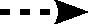
\includegraphics[height=1.0ex]{fig_Dashed}}}\)) relations.
           The ``upstream'' (\(\vcenter{\hbox{\protect
\includegraphics[height=1.0ex]{fig_Backward}}}\))
           and ``downstream'' (\(\vcenter{\hbox{\protect
\includegraphics[height=1.0ex]{fig_Forward}}}\))
           flow of information towards a specific \(\bm{x}_{\analyzed}\) is indicated.
           This is a form of borrowing strength.
          }
  \label{fig:PEM:DAG:CombInf}
\end{figure}

\section{Bayesian computations} \label{sec:PEM:Computations}
%%%%%%%%%%%%%%%%%%%%%%%%%
% BAYESIAN COMPUTATIONS %
%%%%%%%%%%%%%%%%%%%%%%%%%
Generally Bayesian posteriors feature an analytic closed-form expression only on a rare occasion.
Specifically this applies to posteriors of the form \cref{eq:PEM:Multilevel:Inference:JointPosterior,eq:PEM:Multilevel:Marginal:Posterior,eq:PEM:Multilevel:PerfectData:Posterior}.
% MARKOV CHAIN MONTE CARLO
Notwithstanding the above, posteriors can be explored by means of Markov chain Monte Carlo (MCMC) \cite{MCMC:Gilks1996,MCMC:Robert2004}.
Principally this readily refers to posteriors stemming from multilevel inversion.
% MH & GIBBS SAMPLING
The Metropolis-Hastings (MH) algorithm and the Gibbs sampler are prototypical MCMC techniques.
% SECTION OUTLINE
In \cref{sec:PEM:Computations:MH} we will review the MH algorithm and discuss classical MCMC key issues in \cref{sec:PEM:Computations:KeyChallenges}.
Additional computational key challenges posed by Bayesian multilevel model calibration will be discussed in \cref{sec:PEM:Computations:MultilevelChallenges}.
Some more sophisticated MCMC samplers that are suitable in a multilevel-context are surveyed in \cref{sec:PEM:Computations:AdvancedSamplers}.

\subsection{The Metropolis-Hastings algorithm} \label{sec:PEM:Computations:MH}
% MCMC PRINCIPLE
MCMC is based on constructing an ergodic Markov chain such that its invariant distribution equals the posterior.
% METROPOLIS-HASTINGS
Let \(\pi(\bm{q})\) be the prior and \(\pi(\bm{q} \cond \tuple{\bm{y}_i})\) the posterior density of some QoI \(\bm{q}\).
A Markov chain with equilibrium distribution \(\pi(\bm{q} \cond \tuple{\bm{y}_i})\) is generated by initializing at \(\bm{q}^{(0)}\) and repetitively proceeding as follows.
Given a state \(\bm{q}^{(t)}\) that the Markov chain has taken on in some iteration, in the following iteration a candidate state
\(\bm{q}^{(\star)} \sim P(\bm{q}^{(\star)} \cond \bm{q}^{(t)})\) is randomly sampled from a proposal distribution \(P(\bm{q}^{(\star)} \cond \bm{q}^{(t)})\).
In the MH correction step the proposed state is approved as the new state \(\bm{q}^{(t+1)} = \bm{q}^{(\star)}\) of the Markov chain with probability
\begin{equation} \label{eq:PEM:MCMC:MHCorrection}
  \alpha \left( \bm{q}^{(\star)}, \bm{q}^{(t)} \right)
  \, = \, \mathrm{min} \left( 1,\frac{ \pi(\bm{q}^{(\star)} \cond \tuple{\bm{y}_i}) \, P(\bm{q}^{(t)} \cond \bm{q}^{(\star)}) }
                                     { \pi(\bm{q}^{(t)} \cond \tuple{\bm{y}_i}) \, P(\bm{q}^{(\star)} \cond \bm{q}^{(t)})     } \right).
\end{equation}
Otherwise the proposal will be rejected, i.e.\ the Markov chain remains in its state \(\bm{q}^{(t+1)} = \bm{q}^{(t)}\) of the preceding iteration.
% UNSCALED POSTERIOR
It is important to note that due to the MH acceptance probability \cref{eq:PEM:MCMC:MHCorrection}, the algorithm calls for the computation of posterior ratios only.
Thus for MCMC sampling the scale factors in \cref{eq:PEM:Multilevel:Inference:JointPosterior,eq:PEM:Multilevel:Marginal:Posterior,eq:PEM:Multilevel:PerfectData:Posterior}
can be dropped and only unscaled posterior densities have to be evaluated.
\par % SAMPLING SCHEMES
% RANDOM WALK SAMPLING
Random walk Metropolis sampling rests upon local proposals, e.g.\ candidate states are sampled from a Gaussian distribution
\(\bm{q}^{(\star)} \sim \mathcal{N}(\bm{q}^{(\star)} \distparam \bm{q}^{(t)},\bm{\Sigma}_{\bm{q}})\) that is centered around the current state \(\bm{q}^{(t)}\).
The covariance matrix \(\bm{\Sigma}_{\bm{q}}\) determines the ``stepsizes'' of the algorithm.
% INDEPENDENCE SAMPLING
Independence MH sampling is based on nonlocal proposals whose distribution \(\bm{q}^{(\star)} \sim P(\bm{q}^{(\star)})\) is independent of \(\bm{q}^{(t)}\),
e.g.\ sampling candidate states from the prior \(\bm{q}^{(\star)} \sim \pi(\bm{q}^{(\star)})\) or from some suitable approximation of the posterior \(\bm{q}^{(\star)} \sim \hat{\pi}(\bm{q}^{(\star)} \cond \tuple{\bm{y}_i})\).

\subsection{Classical key challenges} \label{sec:PEM:Computations:KeyChallenges}
% MIXING PROPERTIES
The performance of MCMC methods is governed by the mixing properties of the underlying Markov chain, i.e.\ the speed of convergence of the Markov chain towards the targeted posterior.
% AUTOCORRElATION
As to which degree MCMC samples are autocorrelated has a determining influence on the convergence speed and their quality as posterior representatives.
% DESIGN & TUNING
Hence MCMC algorithms are designed and tuned in pursuit of rapid mixing.
Depending on the specific problem at hand, this may be a tricky business which requires to employ and combine sophisticated and highly specialized sampling schemes.
% FORWARD MODEL RUNS
Typically MCMC sampling calls for a high number of program iterations which in turn demands a high number of forward model runs for evaluating the likelihood function in the MH correction \cref{eq:PEM:MCMC:MHCorrection}.
% CONVERGENCE CHECKS
Beyond that, careful convergence diagnostics are of particular importance for MCMC methods.
One has to assess when the Markov chain has reached its stationary distribution, i.e.\ when it has lost any dependence on its initialization.
% ADVANCED DIAGNOSTICS & HEURISTICS
Even though there are advanced convergence test \cite{MCMC:Cowles1996,MCMC:Brooks1998:Roberts},
e.g.\ Gelman-Rubin diagnostics for multiple over-dispersed chains \cite{MCMC:Gelman1992,MCMC:Brooks1998:Gelman},
we remark that from a pessimistic point of view any convergence diagnostic is heuristics \cite{MCMC:Geyer2011:a}.
% HIGH-DIMENSION & MULTIMODALITY
Furthermore MCMC suffers from difficulties in exploring high-dimensional and multimodal posteriors.

\subsection{Multilevel-related challenges} \label{sec:PEM:Computations:MultilevelChallenges}
% MULTILEVEL MCMC
Multilevel posteriors can be readily sampled by means of classical MCMC techniques as they are commonly applied in ``simple'' Bayesian inversion.
However, on top of the classical bottlenecks that were discussed above, one is faced with multilevel-specific MCMC challenges.
% JOINT vs MARGINAL
The posteriors \cref{eq:PEM:Multilevel:Inference:JointPosterior,eq:PEM:Multilevel:Marginal:Posterior}, which are appertain to the joint and the marginal variant of multilevel calibration, are different in nature.
Accordingly, sampling these posteriors pose different computational burdens.
The former requires a sampling scheme that performs efficiently in high-dimensional parameter spaces, whereas the latter suffers from computing the integrated likelihood \cref{eq:PEM:Multilevel:Marginal:Likelihood}.
% PERFECT DATA
Similarly the posterior \cref{eq:PEM:Multilevel:PerfectData:Posterior} of the ``perfect'' data model imposes forward uncertainty quantification for the computation of the likelihood \cref{eq:PEM:Multilevel:PerfectData:Likelihood}.
\par % LIKELIHOOD ESTIMATION
Likelihood functions of the form \cref{eq:PEM:Multilevel:Marginal:LikelihoodEstimator,eq:PEM:Multilevel:PerfectData:LikelihoodEstimator} suffer from another severe difficulty.
% POSTERIOR FIDELITY
It is well-known that statistical estimations of the likelihood ratio introduce an additional random component into the Markov chain transition kernel \cite{MCMC:ONeill2000,MCMC:Bal2013}.
Consequently the steady-state distribution of the chain may be modified.
Therefore free parameters of the algorithm have to be chosen endeavoring high \textit{posterior fidelity},
i.e.\ the degree as to which the induced long-run distribution conforms with the true posterior \cite{Nagel:SciTech2014:Proc,Nagel:JAIS2015}.

\subsection{Advanced MCMC samplers} \label{sec:PEM:Computations:AdvancedSamplers}
% TOTAL NUMBER OF FORWARD MODEL RUNS
Summarized Bayesian multilevel model calibration requires an enormous number of forward model runs.
Therefore in the statistical literature a wide range of advanced MCMC techniques, dedicated to posterior exploration in classical hierarchical models, have been devised.
Some enhanced Gibbs sampling methods in this context are reviewed in \cite{MCMC:Gilks1996} and references therein.
% ENGINEERING APPLICATIONS
However, in view of engineering problems they may not meet the challenges those applications usually pose.
This is due to the inescapable ``blackbox'' character of the forward solver and nonconjugacy.
Generally not all of the parameters will have full conditionals of a standard form that can be easily sampled.
% DA & HMC
Despite that this paper does not focus on computational facets of uncertainty quantification, a short outlook on potentially efficient MCMC implementations is given.
\par % DATA AUGMENTIATON
Data augmentation is a powerful MCMC technique that aims at enhancing the numerical efficiency of posterior computation by introducing missing data as auxiliary variables \cite{MCMC:Dyk2001,MCMC:Dyk2003}.
% NATURALL EMERGENCE
Note that the joint posterior \cref{eq:PEM:Multilevel:Inference:JointPosterior} can be seen as an augmented form of the marginal one in \cref{eq:PEM:Multilevel:Marginal:Posterior}.
Thus data augmentation naturally emerges in the context of Bayesian multilevel inversion.
% PARTIAL DATA AUGMENTATION
It has been beneficially applied for solving multilevel inverse problems within the domain of aerospace engineering \cite{Nagel:SciTech2014:Proc,Nagel:JAIS2015}.
% PSEUDO MARGINALIZATION
Vice versa, there are dedicated MCMC schemes for directly computing marginalized posteriors of the form \cref{eq:PEM:Multilevel:Marginal:Posterior},
e.g.\ MC within Metropolis sampling \cite{MCMC:ONeill2000,MCMC:Beaumont2003} or pseudo-marginalization \cite{MCMC:Andrieu2009}.
% HAMILTONIAN MONTE CARLO
The Hamiltonian Monte Carlo (HMC) algorithm is a sampler whose performance is remarkably efficient in high-dimensional parameter spaces and for highly correlated posteriors \cite{MCMC:Duane1987,MCMC:Neal2011}.
Since multilevel models are higher-dimensional and correlated by definition, the HMC is a promising MCMC candidate in this context.
% (UNDER)ACKNOWLEDGEMENT
Yet the HMC still occurs to be highly underacknowledged in Bayesian inference in general and for hierarchical models in particular.

\section{Numerical case studies} \label{sec:PEM:CaseStudies}
%%%%%%%%%%%%%%%%%%%%%%%%%%
% NUMERICAL CASE STUDIES %
%%%%%%%%%%%%%%%%%%%%%%%%%%
In order to illustrate the power and versatility of the devised framework we conduct a selection of computer experiments.
This shall be seen as a proof of concept and benchmark of the proposed methodology in the context of engineering applications.
% FORWARD PROBLEM: MULTIPLE BEAMS
A system of identically designed structural components functions as the basis for probing a range of experimental scenarios.
Specifically we deal with an ensemble of simply supported beams that are tested in a series of three-point bending experiments.
% INVERSE PROBLEMS UNDER UNCERTAINTY
By multilevel analysis of measured beam deflections we highlight how different inferential goals, e.g.\ probabilistic inversion, residual calibration or optimal combination of information,
can be achieved in the presence of material variability and uncertainties in the experimental setup.
% DETERMINISTIC MODELING
Keeping deterministic modeling simple and intuitive will allow us to focus on uncertainty quantification aspects that are the essential subject matter of this research.
% COMPUTATIONAL OBSTACLES
Incidentally we learn about the computational obstacles that must be overcome when aiming at ``real-world'' applications.
\par % SECTION OUTLINE
The forward problem will be shortly introduced in \cref{sec:PEM:CaseStudies:Beams}.
Around this submodel, that covers the deterministic features of the system, Bayesian multilevel models will be built to capture uncertainty and variability.
Probabilistic inversion, i.e.\ deducing the material variability throughout an ensemble of similar specimens, will be tackled in \cref{sec:PEM:CaseStudies:ProbInv}.
The subsequent \cref{sec:PEM:CaseStudies:ResCal} will deal with residual model calibration.
In \cref{sec:PEM:CaseStudies:AddPres} the impact of prescribed uncertainties in the test conditions will be investigated.
In \cref{sec:PEM:CaseStudies:CombInf} borrowing strength will be utilized in order to ideally estimate the material characteristics of a single specimen by using information obtained from the other specimens.

%%%%%%%%%%%%%%%%%%%%%%%%%%%%%%%%%%%%%%%%%%%%%%%%%%%%%%%%%%%%%%%%%%%%%%%%%%%%%%%%%%%%%%%%%%%%%%%%%%%%%%%%%%%%%%%%%%%%%%%%%%%%%%%%%%%%%%%%%%%%%%%%%%%%%%%%%%%%%%%%%%%%%%%%%%%%%%%%%%%%%%%%%
\subsection{Mechanical model} \label{sec:PEM:CaseStudies:Beams}
%%%%%%%%%%%%%%%%%%%%
% MECHANICAL MODEL %
%%%%%%%%%%%%%%%%%%%%
The system under consideration is an ensemble of identically manufactured beams \(i=1,\ldots,n\) with well-known lengths \(L_i\) and rectangular cross sections with widths \(b_i\) and heights \(h_i\).
Yet the completed beams are only similar in the sense that we assume variability in the elastic moduli \(E_i\) across the ensemble, e.g.\ due to slight irregularities in the fabrication process.
For each single beam \(i\) the Young's modulus \(E_i\) is assumed to be constant along the main beam axis.
% FORWARD FORMULA
The deflections \(\perfect{v}_i(s_{i,j})\) of a simply supported beam \(i\) under a concentrated point load \(F_i\) at midspan can be easily derived in Euler-Bernoulli beam theory.
For positions \(s_{i,j}\) along the beam axis with \(0 \leq s_{i,j} \leq L_i/2\) and \(j=1,\ldots,n_i\) the deflections follow as
\begin{equation} \label{eq:PEM:Beams:AlgebraicFormula}
  \perfect{v}_i(s_{i,j}) = \frac{F_i s_{i,j} }{48 E_i I_i} \left(3 L_i^2 - 4s_{i,j}^2 \right), \;\, \text{for} \;\, 0 \leq s_{i,j} \leq L_i/2,
\end{equation}
where the moment of inertia is given as \(I_i = b_i h_i^3 / 12\).
Likewise a symmetric expression holds for positions \(s_{i,j}\) along the main axis with \(L_i/2 \leq s_{i,j} \leq L_i\).
% SIMPLY SUPPORTED BEAM
A single simply supported beam is visualized in \cref{fig:PEM:Beams:SimpleBeam}.
\begin{figure}[ht]
  \centering
  \includegraphics[width=\PEMbeamWidth]{fig_PEM_SimpleBeam}
  \caption[A simply supported beam]{A simply supported beam.}
  \label{fig:PEM:Beams:SimpleBeam}
\end{figure}
\par % VECTORIZATION
Together with its symmetric counterpart, the algebraic formula \cref{eq:PEM:Beams:AlgebraicFormula} constitutes the deterministic submodel of the system under consideration.
When a load \(F_i\) is applied to a beam \(i\) with physical dimensions \(\bm{l}_i = (L_i,b_i,h_i)\) and an elastic modulus \(E_i\),
these relations predict the deflections \(\perfect{\bm{v}}_i = (\perfect{v}_i(s_{i,1}),\ldots,\perfect{v}_i(s_{i,n_i}))\) at positions \(\bm{s}_i = (s_{i,1},\ldots,s_{i,n_i})\).
We denote this as
\begin{equation} \label{eq:PEM:Beams:ForwardModel}
  \perfect{\bm{v}}_i = \mathcal{M}(E_i,F_i,\bm{l}_i,\bm{s}_i).
\end{equation}
% UNCERTAINTY MODELS
When beam deflections are measured in three-point bending tests for each member \(i=1,\ldots,n\) in the population,
multilevel inversion allows for optimal data analysis in experimental situations where the inputs of \cref{eq:PEM:Beams:ForwardModel} are subject to uncertainty.

%%%%%%%%%%%%%%%%%%%%%%%%%%%%%%%%%%%%%%%%%%%%%%%%%%%%%%%%%%%%%%%%%%%%%%%%%%%%%%%%%%%%%%%%%%%%%%%%%%%%%%%%%%%%%%%%%%%%%%%%%%%%%%%%%%%%%%%%%%%%%%%%%%%%%%%%%%%%%%%%%%%%%%%%%%%%%%%%%%%%%%%%%
\subsection{Probabilistic inversion} \label{sec:PEM:CaseStudies:ProbInv}
%%%%%%%%%%%%%%%%%%%%%%%%%%%
% PROBABILISTIC INVERSION %
%%%%%%%%%%%%%%%%%%%%%%%%%%%
We begin with Bayesian probabilistic inversion, on the basis of which we demonstrate how one can quantify the material variability within the ensemble of beams in a series of bending tests.
A numerical experiment is therefore set up as follows.
% EXPERIMENTAL SETUP
We consider a number of \(n=100\) beams with well-known dimensions \(L_i=\unit[1]{m}\) and \(b_i=h_i=\unit[10]{cm}\).
Beams are subjected to concentrated loads \(F_i=\unit[30]{kN}\) that are applied at midspan.
For \(i=1,\ldots,100\) Young's moduli \(E_i\) are independently sampled from a lognormal distribution \(\mathcal{LN}(E_i \cond \mu_E,\sigma_E)\) with mean \(\mu_E=\unit[15]{GPa}\) and standard deviation \(\sigma_E=\unit[3]{GPa}\).
This corresponds to a coefficient of variation \(c_{E} = \unit[20]{\%}\).
% TREATED AS UNKNOWNS
After having set up the experiment, the hyperparameters \(\bm{\theta}_E=(\mu_E,\sigma_E)\) as well as beam-specific moduli \(E_i\) will be treated as unknowns. 
% PREDICTED DEFLECTIONS
At \(n_i=3\) positions \(\bm{s}_i = (s_{i,1},s_{i,2},s_{i,3})\) with \(s_{i,1}=\unit[25]{cm}\), \(s_{i,2}=\unit[50]{cm}\) and \(s_{i,3}=\unit[75]{cm}\)
beam deflections \(\perfect{\bm{v}}_i = (\perfect{v}_i(s_{i,1}),\perfect{v}_i(s_{i,2}),\perfect{v}_i(s_{i,3}))\) are computed according to \cref{eq:PEM:Beams:AlgebraicFormula}.
% MEASUREMENT UNCERTAINTY
In order to take measurement uncertainty and forward model imperfection into account, we perturb the predictions \(\perfect{\bm{v}}_i\) with noise terms \(\bm{\varepsilon}_i = (\varepsilon_{i,1},\varepsilon_{i,2},\varepsilon_{i,3})\).
Those terms are independently sampled from Gaussian distributions \(\mathcal{N}(\bm{\varepsilon}_i \distparam \bm{0},\bm{\Sigma}_i)\) with \(\bm{\Sigma}_i = \sigma_i^2 \bm{I}_3\) and \(\sigma_i = \unit[0.1]{mm}\).
% PSEUDO DATA & INFERENTIAL GOAL
Eventually \(\bm{v}_i = \perfect{\bm{v}}_i + \bm{\varepsilon}_i\) represent the pseudo data that will become analyzed with respect to the QoI \(\bm{\theta}_E = (\mu_E,\sigma_E)\).
\par % HYPERPRIOR MODEL
In many circumstances expert knowledge about the QoI \(\bm{\theta}_E\) is available prior to analyzing the data.
This knowledge can be accounted for by eliciting a suitable prior distribution \(\pi(\bm{\theta}_E)\).
Herein we employ a proper Bayesian prior \(\pi(\bm{\theta}_E) = \pi(\mu_E) \, \pi(\sigma_E)\) with independent marginals.
As measured in units of \(\unit[]{GPa}\) those marginals are given as uniform distributions \(\pi(\mu_E) = \mathcal{U}(0,100)\) and \(\pi(\sigma_E) = \mathcal{U}(0,30)\).
This is supposed to represent an experimental situation where one cannot elicit informative priors, nonetheless one is confident enough to assign this weakly informative and flat prior with its upper and lower bounds.
\par % PROBABILISTIC INVERSION
Ultimately probabilistic inversion can be summarized as the estimation of the QoI \(\bm{\theta}_{\bm{X}} \equiv \bm{\theta}_E\) with the deflection measurements \(\tuple{\bm{y}_i} \equiv \tuple{\bm{v}_i}\).
Beam-specific Young's moduli \(\tuple{\bm{x}_i} \equiv \tuple{E_i}\), that are not of immediate inferential interest, are considered nuisance to that end.
Experimental conditions \(\tuple{\bm{d}_i} \equiv \tuple{(F_i,\bm{l}_i,\bm{s}_i)}\), that the experiments where subject to, and prediction error models \(\tuple{\bm{\Sigma}_i}\) are assumed to be known.
The distributions \(f_{\bm{X} \cond \bm{\Theta}_{\bm{X}}} (\bm{x}_i \cond \bm{\theta}_{\bm{X}}) \equiv \mathcal{LN}(E_i \cond \mu_E,\sigma_E)\) and
\(\pi_{\bm{\Theta}_{\bm{X}}}(\bm{\theta}_{\bm{X}}) \equiv \pi(\bm{\theta}_E)\) represent the available structural and parametric prior knowledge, respectively.
The emerging posterior will be of the form \(\pi( \bm{\theta}_{\bm{X}} \cond \tuple{\bm{y}_i}) \equiv \pi( \bm{\theta}_E \cond \tuple{\bm{v}_i})\).
It can be directly sampled or accessed via the QoI-marginals of the joint posterior \(\pi( \tuple{\bm{x}_i},\bm{\theta}_{\bm{X}} \cond \tuple{\bm{y}_i}) \equiv \pi( \tuple{E_i},\bm{\theta}_E \cond \tuple{\bm{v}_i})\).
% DAG
A DAG corresponding to probabilistic inversion is provided in \cref{fig:PEM:DAG:ProbInv}.

\subsubsection{MCMC}
% JOINT VS. MARGINAL
Generally we employ a joint rather than a marginal problem formulation.
% EXACT POSTERIOR SAMPLING
For the fidelity reasons that were discussed in \cref{sec:PEM:Computations:MultilevelChallenges} this allows for exact posterior computation where an approximation is only introduced in as much as MCMC sampling is concerned.
% ADDITIONAL INSIGHT
Moreover a joint posterior features a richer structure which will provide new insights into multilevel inversion.
% COMPUTER ISSUES
All computations will be serially done on a contemporary Intel Xeon CPU.
\par % MCMC
The joint posterior \(\pi(\tuple{E_i},\bm{\theta}_E \cond \tuple{\bm{v}_i})\) is sampled by means of a blockwise random walk Metropolis algorithm.
% CUMBERSUME TUNING
A practical problem of random walk samplers in high dimension is to carefully tune the proposal distribution.
For complex multivariate posterior distributions this is a cumbersome procedure that poses severe difficulties.
% SYMMETRY CONSIDERATIONS
However, in multilevel inversion one can advantageously exploit the ``symmetry'' of the problem in the latent variables.
Assuming that separate inverse problems \(i\) with \(1 \leq i \leq n\) are not severely ill-posed, latent variables of the same uncertainty type are expected to behave similarly in the sense that their marginal posteriors resemble one another.
Moreover, due to the indirectness of borrowing strength, their mutual correlations are expected to be rather small.
Along these lines the ``effective dimensionality'' is lower than the number of unknowns suggests.
% BLOCKWISE STRUCTURE
This discussion motivates that MCMC updates are done in blocks \(\tuple{E_i}\) and \((\mu_E,\sigma_E)\).
% ACCEPTANCE RATES
We find that with Gaussian jumping distributions the algorithm can be easily tuned in such a way that blockwise acceptance rates range between \(\unit[20]{\%}\) and \(\unit[40]{\%}\).
% INITIALIZATION
Avoiding lengthy convergence times in high-dimensional problems requires smart initialization, too.
Again we proceed by exploiting the structure of the multilevel system.
The block \(\tuple{E_i}\) is initialized with solutions of separate inverse problems, while two-stage estimates are used in the hyperparameter block \((\mu_E,\sigma_E)\).
\par % CONVERGENCE
In order to assure duly completed posterior exploration we perform a number of convergence checks.
The algorithm is initialized in regions of the parameter space that had not been visited before and the convergence behavior of the Markov chain is monitored.
We detect that the chain eventually reaches the same posterior modes again.
% TRACE PLOTS
In \cref{fig:PEM:ProbInv:Chains} trace plots of a converging Markov chain are shown for its \(\mu_E\) and \(\sigma_E\) components.
They have been initialized at \(\mu_E^{(0)}=\unit[50]{GPa}\) and \(\sigma_E^{(0)}=\unit[15]{GPa}\), i.e.\ in the middle of their priorly admissible intervals.
% CONVERGENCE BEHAVIOR
While the mean hyperparameter \(\mu_E\) directly converges as shown in \cref{fig:PEM:ProbInv:Chain:Mean}, we observe a different behavior for the spread hyperparameter \(\sigma_E\).
From \cref{fig:PEM:ProbInv:Chain:Sigma} it can be seen that the latter chain tends to higher values prior to attraction towards the posterior mean.
% INTERPRETATION
For the given initialization this is a systematic effect that indicates a posterior correlation in the hyperparameters \((\mu_E,\sigma_E)\).
Eventually the Markov chain converges within ca.\ \(400\) MCMC iterations.
% ADVANCED DIAGNOSTICS
Apart from such visual inspections we generally rely on Gelman-Rubin diagnostics for parallel chains \cite{MCMC:Gelman1992,MCMC:Brooks1998:Gelman}.
% MARKOV CHAINS
\begin{figure}[ht]
  \centering
  \begin{subfigure}[b]{0.5\textwidth}
    \centering
    \includegraphics[height=\PEMfigHeight]{fig_PEM_ProbInvChainMean}
    \caption{Convergence of \(\mu_E\).}
    \label{fig:PEM:ProbInv:Chain:Mean}
  \end{subfigure}%
  \begin{subfigure}[b]{0.5\textwidth}
    \centering
    \includegraphics[height=\PEMfigHeight]{fig_PEM_ProbInvChainSigma}
    \caption{Convergence of \(\sigma_E\).}
    \label{fig:PEM:ProbInv:Chain:Sigma}
  \end{subfigure}%
  \caption[Trace plots of a converging Markov chain]{Trace plots of a converging Markov chain.
           For \(n=100\) the converging Markov chain is shown for \(\mu_E\) in \subref{fig:PEM:ProbInv:Chain:Mean} and for \(\sigma_E\) in \subref{fig:PEM:ProbInv:Chain:Sigma}.
           Being initialized at \(\mu_E^{(0)}=\unit[50]{GPa}\) and \(\sigma_E^{(0)}=\unit[15]{GPa}\) the Markov chain converges within ca.\ \(400\) MCMC iterations.
           In equilibrium the Markov chain samples the posterior around its mean.
           }
  \label{fig:PEM:ProbInv:Chains}
\end{figure}
\par % AUTOCORRELATION
In \cref{fig:PEM:ProbInv:ACF} the MCMC sample autocorrelations are plotted for the QoI \((\mu_E,\sigma_E)\) and for an intermediate variable \(E_i\) with \(i=1\).
It can be seen how the autocorrelation function (ACF) drops until it becomes indistinguishable from zero.
This behavior governs the quality of the sample as a posterior representative.
Especially the ACF of \(E_i\) shown in \cref{fig:PEM:ProbInv:ACF:Param} motivates more efficient updating schemes in future research.
% AUTOCORRELATION
\begin{figure}[ht]
  \centering
  % MEAN HYPERPARAMETER
  \begin{subfigure}[b]{0.33\textwidth}
    \centering
    \includegraphics[height=\PEMfigHeight]{fig_PEM_ProbInvACFMean}
    \caption{Autocorrelation of \(\mu_E\).}
    \label{fig:PEM:ProbInv:ACF:Mean}
  \end{subfigure}%
  % SIGMA HYPERPARAMETER
  \begin{subfigure}[b]{0.33\textwidth}
    \centering
    \includegraphics[height=\PEMfigHeight]{fig_PEM_ProbInvACFSigma}
    \caption{Autocorrelation of \(\sigma_E\).}
    \label{fig:PEM:ProbInv:ACF:Sigma}
  \end{subfigure}%
  % INDIVIDUAL PARAMETER
  \begin{subfigure}[b]{0.33\textwidth}
    \centering
    \includegraphics[height=\PEMfigHeight]{fig_PEM_ProbInvACFParam}
    \caption{Autocorrelation of \(E_1\).}
    \label{fig:PEM:ProbInv:ACF:Param}
  \end{subfigure}%
  \caption[Sample autocorrelation functions]{Sample autocorrelation functions.
           For a run with \(n=100\) the MCMC sample autocorrelation function is plotted for \(\mu_E\) in \subref{fig:PEM:ProbInv:ACF:Mean},
           for \(\sigma_E\) in \subref{fig:PEM:ProbInv:ACF:Sigma} and for \(E_1\) in \subref{fig:PEM:ProbInv:ACF:Param}.
           The sample autocorrelation determines the effective MCMC sample size.
           }
  \label{fig:PEM:ProbInv:ACF}
\end{figure}

\subsubsection{Results: Posterior marginals}
% ANALYZED DATA
We analyze the data \(\tuple{\bm{v}_i}_{1\leq i \leq 100}\) as well as its subconfigurations \(\tuple{\bm{v}_i}_{1 \leq i \leq 10}\), \(\tuple{\bm{v}_i}_{1\leq i \leq 20}\) and \(\tuple{\bm{v}_i}_{1\leq i \leq 50}\).
This allows to assess how the number of experiments \(n\) influences the identification of the QoI.
% MCMC ITERATIONS
For each of the runs \(N=10^7\) MCMC iterations are performed.
% BURN-IN
As a general rule we discard the initial \(\unit{1}{\%}\) of the total number of iterations of each Markov chain as a burn-in period.
% COMPUTATION TIME
The total algorithm runtime adds up to \(t=\unit[3.85]{h}\) for \(n=10\) and to \(t=\unit[4.66]{h}\) for \(n=100\).
% POSTERIOR MARGINALS
The resulting posterior marginals of \(\mu_E\) and \(\sigma_E\) are shown in \cref{fig:PEM:ProbInv:Marginals}.
% TABLE
A statistical summary of these marginals can be found in \cref{tab:PEM:ProbInf:Summary}, where the mean, mode, standard deviation (SD) and coefficient of variation (CV) are listed.
% REMARKS
With increasing number of processed experiments \(n\),
Bayesian point estimates (mean, mode) approach the true values \(\mu_E = \unit[15]{GPa}\) and \(\sigma_E = \unit[3]{GPa}\) while measures of estimation uncertainty (SD, CV) expectedly decrease.
% MARGINAL POSTERIORS
\begin{figure}[ht]
  \centering
  \begin{subfigure}[b]{0.5\textwidth}
    \centering
    \includegraphics[height=\PEMfigHeight]{fig_PEM_ProbInvPostMean}
    \caption{Posterior marginal of \(\mu_E\).}
    \label{fig:PEM:ProbInv:Post:Mean}
  \end{subfigure}%
  \begin{subfigure}[b]{0.5\textwidth}
    \centering
    \includegraphics[height=\PEMfigHeight]{fig_PEM_ProbInvPostSigma}
    \caption{Posterior marginal of \(\sigma_E\).}
    \label{fig:PEM:ProbInv:Post:Sigma}
  \end{subfigure}%
  \caption[Posterior marginals of the QoI]{Posterior marginals of the QoI.
           Corresponding to various numbers of experiments \(n\), the marginal posterior densities of \(\mu_E\) and \(\sigma_E\)
           are shown in \subref{fig:PEM:ProbInv:Post:Mean} and \subref{fig:PEM:ProbInv:Post:Sigma}, respectively.
           For increasing \(n\), the posterior uncertainty in estimating the QoI \(\bm{\theta}_E = (\mu_E,\sigma_E)\)
           with \(\mu_E=\unit[15]{GPa}\) and \(\sigma_E = \unit[3]{GPa}\) steadily decreases.
          }
  \label{fig:PEM:ProbInv:Marginals}
\end{figure}
% TABLE: PROBABILISTIC INVERSION
\begin{table}[ht]
  \caption[Summary of the QoI posterior marginals]{Summary of the QoI posterior marginals.}
  \label{tab:PEM:ProbInf:Summary}
  \centering
  \begin{tabular}{lcccccccccc}
    \toprule
    & \phantom{} & \multicolumn{3}{c}{\(\mu_E\) \(\lbrack\unit[]{GPa}\rbrack\)} & \(\lbrack \unitless \rbrack\)
    & \phantom{} & \multicolumn{3}{c}{\(\sigma_E\) \(\lbrack\unit[]{GPa}\rbrack\)} & \(\lbrack \unitless \rbrack\) \\
    \cmidrule{3-6} \cmidrule{8-11}
    && Mean & Mode & SD & CV && Mean & Mode & SD & CV \\
    \midrule
    \(n=10\)  && \(15.98\) & \(15.43\) & \(2.06\) & \(0.13\) && \(4.73\) & \(3.54\) & \(3.55\) & \(0.75\) \\
    \(n=20\)  && \(15.48\) & \(15.36\) & \(0.74\) & \(0.05\) && \(3.18\) & \(2.90\) & \(0.65\) & \(0.20\) \\
    \(n=50\)  && \(15.20\) & \(15.17\) & \(0.46\) & \(0.03\) && \(3.17\) & \(3.08\) & \(0.37\) & \(0.12\) \\
    \(n=100\) && \(15.02\) & \(15.00\) & \(0.30\) & \(0.02\) && \(3.02\) & \(2.97\) & \(0.24\) & \(0.08\) \\
    \bottomrule
  \end{tabular}
\end{table}

\subsubsection{Results: Two-dimensional posteriors}
% 2D POSTERIOR
Showing posterior marginals may hide possibly existing dependency structures or the lack thereof.
Those constitute a substantial result of Bayesian data analysis, though.
Hence \cref{fig:PEM:ProbInv:2DPosterior} shows two-dimensional posteriors where interesting correlation properties were discovered.
% HYPERPARAMETERS
The two-dimensional posterior of \((\mu_E,\sigma_E)\) is plotted in \cref{fig:PEM:ProbInv:2DPosterior:MeanSigma}.
According to the posterior probability model these two parameters are correlated with a linear Pearson coefficient of correlation \(r_{\mu_E,\sigma_E}=0.40\).
Note that these parameters were assumed to be independent in accord with their prior model.
% JOINT POSTERIOR
The joint posterior \cref{eq:PEM:ProbInv:JointPosterior} can also feature a correlation between hyperparameters and experiment-specific parameters.
In \cref{fig:PEM:ProbInv:2DPosterior:MeanParam,fig:PEM:ProbInv:2DPosterior:ParamParam} the two-dimensional posteriors of \((\mu_E,E_i)\) and \((E_{j},E_{i})\) with \(i=50\) and \(j=75\) are imaged.
% 2D POSTERIORS
\begin{figure}[ht]
  \centering
  \begin{subfigure}[b]{0.33\textwidth}
    \centering
    \includegraphics[height=\PEMfigHeight]{fig_PEM_ProbInvPost2DMeanSigma}
    \caption{2D posterior of \((\mu_E,\sigma_E)\).}
    \label{fig:PEM:ProbInv:2DPosterior:MeanSigma}
  \end{subfigure}%
  \begin{subfigure}[b]{0.33\textwidth}
    \centering
    \includegraphics[height=\PEMfigHeight]{fig_PEM_ProbInvPost2DMeanParam}
    \caption{2D posterior of \((\mu_E,E_{50})\).}
    \label{fig:PEM:ProbInv:2DPosterior:MeanParam}
  \end{subfigure}%
  \begin{subfigure}[b]{0.33\textwidth}
    \centering
    \includegraphics[height=\PEMfigHeight]{fig_PEM_ProbInvPost2DParamParam}
    \caption{2D posterior of \((E_{75},E_{50})\).}
    \label{fig:PEM:ProbInv:2DPosterior:ParamParam}
  \end{subfigure}%
  \caption[2D posteriors of \((\mu_E,\sigma_E)\), \((\mu_E,E_{50})\) and \((E_{75},E_{50})\)]{2D posteriors of \((\mu_E,\sigma_E)\), \((\mu_E,E_{50})\) and \((E_{75},E_{50})\).
           The two-dimensional posteriors of \((\mu_E,\sigma_E)\), \((\mu_E,E_{50})\) and \((E_{75},E_{50})\) are shown.
           Being priorly independent the components \(\mu_E\) and \(\sigma_E\) are seen to be correlated a posteriori.
           The linear Pearson coefficient of correlation amounts to \(r_{\mu_E,\sigma_E}=0.40\).
           }
  \label{fig:PEM:ProbInv:2DPosterior}
\end{figure}

%%%%%%%%%%%%%%%%%%%%%%%%%%%%%%%%%%%%%%%%%%%%%%%%%%%%%%%%%%%%%%%%%%%%%%%%%%%%%%%%%%%%%%%%%%%%%%%%%%%%%%%%%%%%%%%%%%%%%%%%%%%%%%%%%%%%%%%%%%%%%%%%%%%%%%%%%%%%%%%%%%%%%%%%%%%%%%%%%%%%%%%%%
\subsection{Residual calibration} \label{sec:PEM:CaseStudies:ResCal}
%%%%%%%%%%%%%%%%%%%%%%%%
% RESIDUAL CALIBRATION %
%%%%%%%%%%%%%%%%%%%%%%%%
There are situations where the strong assumption of known residual variances \(\bm{\Sigma}_i = \sigma_i^2 \bm{I}_3\) is somewhat restrictive.
Thus we generalize multilevel inversion as in \cref{sec:PEM:CaseStudies:ProbInv} by treating \(\sigma_{\mathcal{E}} \equiv \sigma_i\) as a global unknown.
% PRIOR MODEL
In units of \(\unit[]{mm}\) the corresponding parametric prior is set to a uniform distribution \(\pi(\sigma_{\mathcal{E}}) = \mathcal{U}(0,0.5)\).
% EXPERIMENTAL SETUP
Otherwise the experimental setup of probabilistic inversion is used.
\par % INFERENTIAL MECHANISM
The standard deviation \(\sigma_{\mathcal{E}}\) of the residual model \(\mathcal{N}(\bm{\varepsilon}_i \cond \bm{0},\sigma_{\mathcal{E}}^2 \bm{I}_3)\)
is introduced as an extra unknown in the model \cref{eq:PEM:ProbInv:Model} and in the posterior \cref{eq:PEM:ProbInv:JointPosterior}.
% PRIOR & POSTERIOR
Consequently the joint prior is given as \(\pi(\tuple{E_i},\mu_E,\sigma_E,\sigma_{\mathcal{E}}) = \pi(\sigma_{\mathcal{E}}) \, \pi(\mu_E) \, \pi(\sigma_E) \prod_{i=1}^n \mathcal{LN}(E_i \cond \mu_E,\sigma_E)\).
For the joint likelihood function one has \(\mathcal{L}(\tuple{E_i},\sigma_{\mathcal{E}} \distparam \tuple{\bm{v}_i}) = \prod_{i=1}^n \mathcal{N}(\bm{v}_i \allowbreak \cond \mathcal{M}(E_i,F_i,\bm{l}_i,\bm{s}_i),\sigma_{\mathcal{E}}^2 \bm{I}_3)\).
Brought together this leads to a joint posterior density that has the shape
\(\pi(\tuple{E_i},\mu_E,\sigma_E, \allowbreak \sigma_{\mathcal{E}} \cond \tuple{\bm{v}_i}) \propto \mathcal{L}(\tuple{E_i},\sigma_{\mathcal{E}} \distparam \tuple{\bm{v}_i}) \, \pi(\tuple{E_i},\mu_E,\sigma_E,\sigma_{\mathcal{E}})\).
\par % MCMC
We sample from this posterior by appending a block for the additional unknown \(\sigma_{\mathcal{E}}\) in the MCMC updating scheme.
In order to assess the influence of the amount of data on the final results, independent runs are performed for \(n = 10\), \(20\), \(50\) and \(100\).
% RESULTS
In \cref{fig:PEM:ResCal:Post:Mean} the relevant posterior marginals for the inference of the residual model \(\sigma_{\mathcal{E}}\) are shown.
A short summary of the these marginals is provided in \cref{tab:PEM:ResCal:Summary}.
% OBSERVATION & INTERPRETATION
The higher the number of analyzed experiments \(n\), the better the true value \(\sigma_{\mathcal{E}} = \unit[0.1]{mm}\) has been revealed.
This proves that one can indeed estimate the parameters of the prediction error model in the context of multilevel calibration.
If this is not of interest for its own sake, it still avoids the requirement of perfect knowledge of the error variance.
% PROBABILISTIC INVERSION
In addition we observed that introducing an uncertainty in the residual model hardly affects the inference of the QoI in probabilistic inversion.
% MARGINAL POSTERIORS: FIGURE & SUMMARY
\begin{figure}[ht]
  \centering
  % MARGINAL POSTERIORS: RESIDUAL SIGMA
  \begin{minipage}[c]{0.52\textwidth}
    \centering
    \includegraphics[height=\PEMfigHeight]{fig_PEM_ResCalPostResidualSigma}
    \captionof{figure}[Posterior marginals of \(\sigma_{\mathcal{E}}\)]{Posterior marginals of \(\sigma_{\mathcal{E}}\).
    The marginal posterior of \(\sigma_{\mathcal{E}}\) is shown for different numbers of data \(n\).
    }
    \label{fig:PEM:ResCal:Post:Mean}
  \end{minipage}%
  \hfill%
  % TABLE: RESIDUAL CALIBRATION
  \begin{minipage}[c]{0.46\textwidth}
    \captionof{table}[Summary of the \(\sigma_{\mathcal{E}}\)-marginals]{Summary of the \(\sigma_{\mathcal{E}}\)-marginals.}
    \label{tab:PEM:ResCal:Summary}
    \centering
    \begin{tabular}{lrrrrr}
      \toprule
      & \phantom{} & \multicolumn{3}{c}{\(\sigma_{\mathcal{E}}\) \(\lbrack\unit[10^{-5}]{m}\rbrack\)} & \multicolumn{1}{c}{\(\lbrack \unitless \rbrack\)} \\
      \cmidrule{3-6}
      && \multicolumn{1}{c}{Mean} & \multicolumn{1}{c}{Mode} & \multicolumn{1}{c}{SD} & \multicolumn{1}{c}{CV} \\
      \midrule
      \(n=10\)  && \(11.00\) & \(10.23\) & \(1.90\) & \(0.17\) \\
      \(n=20\)  && \(8.68\)  & \(8.38\)  & \(1.01\) & \(0.12\) \\
      \(n=50\)  && \(10.65\) & \(10.50\) & \(0.77\) & \(0.07\) \\
      \(n=100\) && \(9.97\)  & \(9.90\)  & \(0.50\) & \(0.05\) \\
      \bottomrule
    \end{tabular}
  \end{minipage}%
\end{figure}

%%%%%%%%%%%%%%%%%%%%%%%%%%%%%%%%%%%%%%%%%%%%%%%%%%%%%%%%%%%%%%%%%%%%%%%%%%%%%%%%%%%%%%%%%%%%%%%%%%%%%%%%%%%%%%%%%%%%%%%%%%%%%%%%%%%%%%%%%%%%%%%%%%%%%%%%%%%%%%%%%%%%%%%%%%%%%%%%%%%%%%%%%
\subsection{Uncertain conditions} \label{sec:PEM:CaseStudies:AddPres}
%%%%%%%%%%%%%%%%%%%%%%%
% ADDITIONAL NUISANCE %
%%%%%%%%%%%%%%%%%%%%%%%
In the following we describe an experimental situation where the inference of the QoI \(\bm{\theta}_E\) is hampered by additional uncertainties in the experimental conditions.
Experimental conditions are formally treated as nuisance parameters with prescribed uncertainties.
More specifically, we do not assume that the loads \(F_i\) are perfectly known anymore.
In contrast, we assume that they are \(\bm{\zeta}_i\)-type variables, i.e.\ they are uncertain yet they follow a known distribution.
% EXPERIMENTAL SITUATION
This represents a well-known situation where the loads \(F_i\) that the testing machine actually applies can only be imprecisely adjusted.
In fact, while a targeted load in each experiment is chosen, the physically realized load \(F_i\) may be uncertain.
This is accounted for by a prescribed distribution \(\mathcal{N}(F_i \distparam \mu_{F_i},\sigma_{F_i}^2)\)
where \(\mu_{F_i}\) is the targeted load and \(\sigma_{F_i}\) represents the degree of uncertainty that is inherent to the test machinery.
\par % NUMERICAL SETUP
The setup for conducting a numerical experiment is similar to the one specified in \cref{sec:PEM:CaseStudies:ProbInv}.
For \(n=50\) beams we set the beam dimensions \(\bm{l}_i\) and measurement positions \(\bm{s}_i\) as before.
Elastic moduli \(E_i\) are randomly drawn from \(\mathcal{LN}(E_i \cond \mu_E,\sigma_E)\) as previously detailed.
In contrast to plain probabilistic inversion, for \(i=1,\ldots,n\) experiment-specific loads \(F_i\) are independently sampled from
normal distributions \(\mathcal{N}(F_i \distparam \mu_{F_i},\sigma_{F_i}^2)\) with \(\mu_{F_i} = \unit[30]{kN}\) and \(\sigma_{F_i} = \unit[3]{kN}\).
This equates to a coefficient of variation \(c_{F_i} = \unit[10]{\%}\).
% COMMENTS
Note that such a high degree of uncertainty is unlikely to be encountered in a real-case experiment.
It is used here to accentuate the results presented below, though.
% TREATED AS UNKNOWNS
The realized loads \(F_i\) will be treated as unknowns whereas the hyperparameters \(\bm{\theta}_{F_i} = (\mu_{F_i},\sigma_{F_i})\), i.e.\ the targeted load and its uncertainty, will be treated as knowns.
% PSEUDO MEASUREMENTS
In accordance with \cref{eq:PEM:Beams:AlgebraicFormula} synthetic measurements \(\bm{v}_i = \perfect{\bm{v}}_i + \bm{\varepsilon}_i\) are generated again.
% HYPERPRIORS
The prior distribution \(\pi(\bm{\theta}_E) = \pi(\mu_E) \, \pi(\sigma_E)\) is also chosen as previously stated.
\par % SUMMARY
The problem of probabilistic inversion under additional prescribed nuisance reads as follows.
The hyperparameters \(\bm{\theta}_{\bm{X}} \equiv \bm{\theta}_E\) are the QoI
whereas experiment-specific unknowns \(\tuple{\bm{x}_i} \equiv \tuple{E_i}\) and \(\tuple{\bm{\zeta}_i} \equiv \tuple{F_i}\) are considered nuisance.
With measurements \(\tuple{\bm{y}_i} \equiv \tuple{\bm{v}_i}\) the QoI can be inferred.
Experimental-specific knowns consist of the hyperparameters \(\tuple{\bm{\theta}_{\bm{Z}_i}} \equiv \tuple{\bm{\theta}_{F_i}}\),
the experimental conditions \(\tuple{\bm{d}_i} \equiv \tuple{(\bm{l}_i,\bm{s}_i)}\) and the residual covariances \(\tuple{\bm{\Sigma}_i}\).
Parametric Bayesian prior knowledge is given by \(\pi_{\bm{\Theta}_{\bm{X}}}(\bm{\theta}_{\bm{X}}) \equiv \pi(\bm{\theta}_E)\)
whereas \(f_{\bm{X} \cond \bm{\Theta}_{\bm{X}}} (\bm{x}_i \cond \bm{\theta}_{\bm{X}}) \equiv \mathcal{LN}(E_i \cond \mu_E,\sigma_E)\) and 
\(f_{\bm{Z}}(\bm{\zeta}_i \distparam \bm{\theta}_{\bm{Z}_i}) \equiv \mathcal{N}(F_i \distparam \mu_{F_i},\sigma_{F_i}^2)\) are structural prior distributions.
Within a joint approach a posterior of the form \(\pi( \tuple{\bm{x}_i},\tuple{\bm{\zeta}_i},\bm{\theta}_{\bm{X}} \cond \tuple{\bm{y}_i}) \equiv \pi( \tuple{E_i},\tuple{F_i},\bm{\theta}_E \cond \tuple{\bm{v}_i})\) arises.
Eventually one is interested in the QoI-marginals \( \pi(\bm{\theta}_{\bm{X}} \cond \tuple{\bm{y}_i}) \equiv \pi(\bm{\theta}_E \cond \tuple{\bm{v}_i})\) only.
% DAG
A DAG corresponding to this experimental situation is shown in \cref{fig:PEM:DAG:AddPres}.

\subsubsection{Results: Hyperparameters}
% PROBLEM FORMULATIONS
We sample the joint posterior \(\pi(\tuple{E_i},\tuple{F_i},\bm{\theta}_E \cond \tuple{\bm{v}_i})\) where nuisance variables \(\tuple{F_i}\) are explicitly accounted for.
% BLOCKSWISE MCMC
In a blockwise manner MCMC sweeps are accomplished for \((\mu_E,\sigma_E)\), \(\tuple{E_i}\) and \(\tuple{F_i}\) which constitute different blocks.
Blockwise proposal distributions are again adjusted in order to obtain acceptance rates in between \(\unit[20]{\%}\) and \(\unit[40]{\%}\).
% INITIALIZATION
Each \(F_i\) in the block \(\tuple{F_i}\) is initialized at \(F_i^{(0)} = \mu_{F_i}\), i.e.\ the structural prior mean.
% CONVERGENCE CHECKS
Other than that initialization, convergence checks and burn-in are accomplished as before.
% COMPUTATION TIME
For \(N=10^7\) MCMC iterations the total computation time amounts to \(t=\unit[7.18]{h}\).
% POSTERIOR MARGINALS
The resulting posterior marginals of \(\mu_E\) and \(\sigma_E\) can be seen in \cref{fig:PEM:AddPres:Marginals}.
A statistical summary is provided in \cref{tab:PEM:AddPres:Summary} where the mean, mode, SD and CV of the marginals are itemized.
% MARGINAL POSTERIORS
\begin{figure}[ht]
  \centering
  \begin{subfigure}[b]{0.5\textwidth}
    \centering
    \includegraphics[height=\PEMfigHeight]{fig_PEM_AddPresPostMean}
    \caption{Posterior marginal of \(\mu_E\).}
    \label{fig:PEM:AddPres:Post:Mean}
  \end{subfigure}%
  \begin{subfigure}[b]{0.5\textwidth}
    \centering
    \includegraphics[height=\PEMfigHeight]{fig_PEM_AddPresPostSigma}
    \caption{Posterior marginal of \(\sigma_E\).}
    \label{fig:PEM:AddPres:Post:Sigma}
  \end{subfigure}%
  \caption[Posterior marginals of the QoI]{Posterior marginals of the QoI.
           The marginal posteriors of \(\mu_E\) and \(\sigma_E\) are provided in \subref{fig:PEM:AddPres:Post:Mean} and \subref{fig:PEM:AddPres:Post:Sigma}, respectively.
           Three experimental scenarios are investigated: the proper treatment of the additional uncertainty, 
           an idealized situation where one would precisely know the loads, and the case of a parsimonious model where the uncertainty remains unrecognized.
          }
  \label{fig:PEM:AddPres:Marginals}
\end{figure}
% TABLE: ADDITIONAL PRESCRIPTION
\begin{table}[ht]
  \caption[Summary of the QoI posterior marginals]{Summary of the QoI posterior marginals.}
  \label{tab:PEM:AddPres:Summary}
  \centering
  \begin{tabular}{lcccccccccc}
    \toprule
      & \phantom{} & \multicolumn{3}{c}{\(\mu_E\) \(\lbrack\unit[]{GPa}\rbrack\)} & \(\lbrack \unitless \rbrack\)
      & \phantom{} & \multicolumn{3}{c}{\(\sigma_E\) \(\lbrack\unit[]{GPa}\rbrack\)} & \(\lbrack \unitless \rbrack\) \\
    \cmidrule{3-6} \cmidrule{8-11}
    && Mean & Mode & SD & CV && Mean & Mode & SD & CV \\
    \midrule
    Proper treatment   && \(15.47\) & \(15.41\) & \(0.51\) & \(0.03\) && \(3.17\) & \(3.05\) & \(0.46\) & \(0.14\) \\
    Oracle scenario    && \(15.16\) & \(15.13\) & \(0.47\) & \(0.03\) && \(3.26\) & \(3.15\) & \(0.39\) & \(0.12\) \\
    Ignorance scenario && \(15.65\) & \(15.60\) & \(0.52\) & \(0.03\) && \(3.61\) & \(3.51\) & \(0.43\) & \(0.12\) \\
    \bottomrule
  \end{tabular}
\end{table}
\par % POSTERIOR SIGNIFICANCE
We try to assess the impact of the uncertainty that had been introduced in the loads \(F_i\) on the estimation of the QoI \(\bm{\theta}_E = (\mu_E,\sigma_E)\).
To that end we pursue the following two strategies.
% IDEALIZED SITUATION
First of all we estimate the QoI while treating the realized loads \(F_i\) as if they were part of the experiment-specific knowns \(\bm{d}_i\).
This ``what-if'' or ``oracle'' scenario actually describes the hypothetical situation that we met in plain probabilistic inversion.
It does not describe the realistic scenario of uncertain conditions \(\bm{\zeta}_i\) that we are actually investigating.
Yet this way of proceeding sheds light on how the prescribed uncertainty in the loads affects the inference of the QoI.
% INTERPRETATION
For \(N=10^7\) and \(t=\unit[4.33]{h}\) the results to probabilistic inversion are added to \cref{fig:PEM:AddPres:Marginals}.
With respect to this idealized situation, one can reassess the previous results of properly treating the loads as uncertain.
The introduction of the uncertainty in the loads had actually shifted the posterior modes and raised the level of estimation uncertainty accordingly.
\par % UNCERECOGNIZED UNCERTAINTY
Second of all we investigate the case that the uncertainty \(\mathcal{N}(F_i \distparam \mu_{F_i},\sigma_{F_i}^2)\) in the applied loads \(F_i\) is simply disregarded.
Either it has not been recognized by mistake or it has been intentionally dropped by making simplifying assumptions in favor of a parsimonious model.
% MISTREATMENT
Rather than treating the loads as belonging to the unknowns \(\bm{\zeta}_i\), we erroneously treat them as such experimental conditions \(\erroneous{\bm{d}}_i\) that only approximately describe the prevailing conditions \(\bm{d}_i\).
While the data has been created under \(\bm{d}_i\), data analysis is carried out under \(\erroneous{\bm{d}}_i\).
% EXPERIMENTAL SITUATION
This describes a situation where the experimenter targets a load \(\erroneous{F}_i = \mu_{F_i}\), but the testing machine actually realizes \(F_i\).
If this uncertainty \(\mathcal{N}(F_i \distparam \mu_{F_i},\sigma_{F_i}^2)\) is not accounted for or not recognized at all,
the analyst will accomplish inference under the spurious assumption that the loads had taken on their targeted values \(\erroneous{F}_i\) during experiment execution.
% RESULTS & INTERPRETATION
For \(N=10^7\) and \(t=\unit[3.75]{h}\) the resulting posteriors are added to \cref{fig:PEM:AddPres:Marginals}.
Our interpretation is that dropping the uncertainty of \(F_i\) corrupts the estimation of the QoI and results in misleading estimates of posterior uncertainty,
whereas the proper treatment of all uncertainties yields results that are closer to the idealized ``oracle'' scenario.

\subsubsection{Results: Intermediate variables}
\par % FURTHER INSIGHTS
Sampling the joint posterior \(\pi(\tuple{E_i},\tuple{F_i},\bm{\theta}_E \cond \tuple{\bm{v}_i})\) of the entirety of unknowns provides further interesting insights.
% POSTERIOR OF THE LOADS
Apart from the QoI-marginals one can examine the posterior model of experiment-specific loads \(F_i\), notwithstanding that they are considered nuisance.
\cref{fig:PEM:AddPres:Posteriors} contains two different posteriors involving some \(F_i\).
In \cref{fig:PEM:AddPres:Post:1DLoad} the posterior marginal of a pinpoint load \(F_i\) is shown for \(i=23\).
The identification of specifically applied loads \(F_i\) is subject to rather high levels of posterior uncertainty.
% IDENTIFIABILITY
This is an issue of statistical identifiability.
When both \(E_i\) and \(F_i\) are uncertain and various combinations of these can explain the observation \(\bm{v}_i\) equally well, then those combinations \((E_i,F_i)\) cannot be distinguished a posteriori.
Of course, the reason is that only the ratio \(F_i/E_i\) in \cref{eq:PEM:Beams:AlgebraicFormula} can be identified.
% POSTERIOR CORRELATION
It is therefore interesting to investigate the posterior correlation between the load \(F_i\) and the modulus \(E_i\) of an experiment \(i\).
The two-dimensional posterior of \((E_i,F_i)\) for \(i=20\) that is shown in \cref{fig:PEM:AddPres:Post:2DMeanLoad} serves as an example.
Posterior mass is assigned to suitable parameter constellations \((E_i,F_i)\) that well-explain the measurement \(\bm{v}_i\).
As expected the posterior is strongly correlated with a linear coefficient of correlation \(r_{F_{20},E_{20}} = 0.99\).
% POSTERIORS: ADDITIONAL PRESCRIPTION
\begin{figure}[ht]
  \centering
  % MARGINAL POSTERIOR: APPLIED LOAD
  \begin{subfigure}[b]{0.5\textwidth}
    \centering
    \includegraphics[height=\PEMfigHeight]{fig_PEM_AddPresPostLoad}
    \caption{Posterior marginal of \(F_{23}\).}
    \label{fig:PEM:AddPres:Post:1DLoad}
  \end{subfigure}%
  % 2D POSTERIOR: LOAD-MODULUS
  \begin{subfigure}[b]{0.5\textwidth}
    \centering
    \includegraphics[height=\PEMfigHeight]{fig_PEM_AddPresPost2DLoadParam}
    \caption{2D posterior of \((F_{20},E_{20})\).}
    \label{fig:PEM:AddPres:Post:2DMeanLoad}
  \end{subfigure}%
  \caption[Posteriors of intermediate variables]{Posteriors of intermediate variables.
           In \subref{fig:PEM:AddPres:Post:1DLoad} the posterior marginal of \(F_{23}\) and its structural prior
           \(\mathcal{N}(F_{23} \distparam \mu_{F_{23}},\sigma_{F_{23}}^2)\) with \(\mu_{F_{23}}=\unit[30]{kN}\) and \(\sigma_{F_{23}}=\unit[3]{kN}\) are shown.
           The posterior is centered around the actual value \(F_{23} = \unit[27.24]{kN}\).
           The two-dimensional posterior of \((F_{20},E_{20})\) with \(r_{F_{20},E_{20}} = 0.99\) is shown in \subref{fig:PEM:AddPres:Post:2DMeanLoad}.
          }
  \label{fig:PEM:AddPres:Posteriors}
\end{figure}

%%%%%%%%%%%%%%%%%%%%%%%%%%%%%%%%%%%%%%%%%%%%%%%%%%%%%%%%%%%%%%%%%%%%%%%%%%%%%%%%%%%%%%%%%%%%%%%%%%%%%%%%%%%%%%%%%%%%%%%%%%%%%%%%%%%%%%%%%%%%%%%%%%%%%%%%%%%%%%%%%%%%%%%%%%%%%%%%%%%%%%%%%
\subsection{Borrowing strength} \label{sec:PEM:CaseStudies:CombInf}
%%%%%%%%%%%%%%%%%%%%%%
% BORROWING STRENGTH %
%%%%%%%%%%%%%%%%%%%%%%
As pointed out in \cref{sec:PEM:CombInf}, Bayesian multilevel modeling allows for ``optimal combination of information'' or ``borrowing strength''.
Here we demonstrate this inferential mechanism and investigate its underlying flow of information for the previous application example.
% QOI / NUISANCE
The Bayesian model of probabilistic inversion \cref{eq:PEM:ProbInv:Model} is considered.
However, as opposed to probabilistic inversion we declare experiment-specific elastic moduli \(\tuple{E_i}\) as the QoI whereas the hyperparameters \(\bm{\theta}_E\) are considered nuisance.
Herein we highlight the optimal inference of a single \(E_{\analyzed}\) for some \(\analyzed \in \{1,\ldots,n\}\).
\par % EXPERIMENTAL SETUP
The experimental setup is similar to the one described in \cref{sec:PEM:CaseStudies:ProbInv}.
For \(n=50\) beams, elastic moduli \(E_i\) are randomly sampled from \(\mathcal{LN}(E_i \cond \mu_E,\sigma_E)\).
Beam dimensions \(\bm{l}_i\), measurement positions \(\bm{s}_i\) and the applied loads \(F_i\) are chosen as before.
% PREDICTIONS
With \cref{eq:PEM:Beams:AlgebraicFormula} beam deflections \(\perfect{\bm{v}}_i\) are predicted.
% PSEUDO DATA
Synthetic data \(\bm{v}_i = \perfect{\bm{v}}_i + \bm{\varepsilon}_i\) are generated by perturbing the predictions \(\perfect{\bm{v}}_i\) with noise.
For this purpose noise terms \(\bm{\varepsilon}_i\) are independently sampled from Gaussian distributions \(\mathcal{N}(\bm{\varepsilon}_i \distparam \bm{0},\bm{\Sigma}_i)\).
% SYSTEMATIC EFFECTS
We choose \(\bm{\Sigma}_i = \sigma_i^2 \bm{I}_3\) with \(\sigma_i = \unit[0.1]{mm}\) for \(i \neq \analyzed\) and \(\sigma_{\analyzed} = \unit[0.1]{cm}\).
The latter describes a comparably large deviation that differs from the setup of \cref{sec:PEM:CaseStudies:ProbInv}.
This choice serves the purpose of clearly illustrating the inferential mechanism of optimal combination of information.
\par % SUMMARY
Eventually optimal combination of information reads as the following problem.
With noisy data \(\tuple{\bm{y}_i} \equiv \tuple{\bm{v}_i}\) an experiment-specific \(\bm{x}_{\analyzed} \equiv E_{\analyzed}\) has to be ideally estimated, i.e.\ taking all available sources of information into account.
The hyperparameters \(\bm{\theta}_{\bm{X}} \equiv \bm{\theta}_E\) as well as \(\tuple{\bm{x}_{\notanalyzed}} \equiv \tuple{E_{\notanalyzed}}\) are considered nuisance to that end.
Experiment-specific knowns are \(\tuple{\bm{d}_i} \equiv \tuple{(F_i,\bm{l}_i,\bm{s}_i)}\) and \(\tuple{\bm{\Sigma}_i}\).
The resultant posterior will be of the form \(\pi(\bm{x}_{\analyzed} \cond \tuple{\bm{y}_i}) \equiv \pi(E_{\analyzed} \cond \tuple{\bm{v}_i})\).
Subsequent to formulating the joint posterior \(\pi( \tuple{\bm{x}_i},\bm{\theta}_{\bm{X}} \cond \tuple{\bm{y}_i}) \equiv \pi( \tuple{E_i},\bm{\theta}_E \cond \tuple{\bm{v}_i})\), the QoI-marginals can be easily extracted.
% REMAINING SETUP
Other than that, the experimental setup of probabilistic inversion is adopted.
% DAG
Thus the experiment can be visualized by the DAG in \cref{fig:PEM:DAG:ProbInv}, too.

\subsubsection{Results: Information accumulation}
% OUTLINE
We conduct simple updating, sequential filtering and multilevel inversion for estimating \(E_{\analyzed}\), as introduced in \cref{sec:PEM:CombInf}.
%%%%%%%%%%%%%%%%%%%%%%%%%%%%%%%%%%%%%%%%%%%%%%%%%%%%%%%%%%%%%%%%%%%%%%%%%%%%%%%%%%%%%%%%%%%%%%%%%%%%%%%%%%%%%%%%%%%%%%%%%%%%%%%%%%%%%%%%%%%%%%%%%%%%%%%%%%%%%%%%%%%%%%%%%%%%%%%%%%%%%%%%%
% SIMPLE UPDATING
First of all we start with the simple Bayesian updating approach that was introduced in \cref{sec:PEM:CombInf:SimpleUpdating}.
% METHOD OF COMPOSITION
By the method of composition we draw \(K = 10^5\) samples \((E_{\analyzed}^{(1)},\ldots,E_{\analyzed}^{(K)})\) from the mixture prior \(\pi(E_{\analyzed})\) that corresponds to \cref{eq:PEM:CombInf:SimpleUpdating:Prior}.
% KDE
With this sample the mixture prior can be evaluated as the corresponding one-dimensional KDE with Gaussian kernel functions.
% POSTERIOR
The posterior \(\pi(E_{\analyzed} \cond \bm{v}_{\analyzed})\) results from conditioning on the piece of data \(\bm{v}_{\analyzed}\).
% MCMC
This univariate posterior is explored in \(N=10^5\) MCMC iterations for which the program execution time amounts to \(t=\unit[5.86]{h}\).
The final result of this simple updating approach is shown in \cref{fig:PEM:CombInf:SimpleUpdating}.
%%%%%%%%%%%%%%%%%%%%%%%%%%%%%%%%%%%%%%%%%%%%%%%%%%%%%%%%%%%%%%%%%%%%%%%%%%%%%%%%%%%%%%%%%%%%%%%%%%%%%%%%%%%%%%%%%%%%%%%%%%%%%%%%%%%%%%%%%%%%%%%%%%%%%%%%%%%%%%%%%%%%%%%%%%%%%%%%%%%%%%%%%
\par % SEQUENTIAL FILTERING
Second of all we conduct the sequential Bayesian filtering program that was proposed in \cref{sec:PEM:CombInf:SequentialFiltering}.
% MCMC % PROBABILISTIC INVERSION
In \(N=10^7\) MCMC iterations that take \(t=\unit[3.95]{h}\), probabilistic inversion for estimating \(\bm{\theta}_E\) is executed with the data \(\tuple{\bm{v}_{\notanalyzed}}\).
% METHOD OF COMPOSITION
MCMC samples from the resultant posterior \(\pi(\bm{\theta}_E \cond \tuple{\bm{v}_{\notanalyzed}})\) are used to sample the compound distribution
\(\pi(E_{\analyzed} \cond \tuple{\bm{v}_{\notanalyzed}})\) in \cref{eq:PEM:CombInf:SequentialFiltering:Prior} via the composition method.
% MIXTURE PRIOR
Subsequently a lognormal fit to these samples acts as the prior for \(E_{\analyzed}\).
% POSTERIOR
This prior and the arising posterior distribution \(\pi(E_{\analyzed} \cond \tuple{\bm{v}_{\notanalyzed}},\bm{v}_{\analyzed})\) are plotted in \cref{fig:PEM:CombInf:SequentialFiltering}.
% MCMC
In \(t = \unit[0.01]{h}\) of execution time \(N=10^5\) MCMC samples of the univariate posterior were sampled.
% INTERPRETATION
By comparison of the two posteriors in \cref{fig:PEM:CombInf:UpdatingAndFiltering}, the shrinkage of the posterior uncertainty from
\(\pi(E_{\analyzed} \cond \bm{v}_{\analyzed})\) to \(\pi(E_{\analyzed} \cond \tuple{\bm{v}_{\notanalyzed}},\bm{v}_{\analyzed})\) becomes apparent.
Both posteriors follow from conditioning on the data \(\bm{v}_{\analyzed}\), they update different priors \(\pi(E_{\analyzed})\) and \(\pi(E_{\analyzed} \cond \tuple{\bm{v}_{\notanalyzed}})\), though.
% FLOW OF INFORMATION
In the first place this proves that Bayesian priors are a valid source of information.
Moreover, this principally shows how learning about \(E_{\analyzed}\) can be indirectly supported by the evidence that \(\tuple{\bm{v}_{\notanalyzed}}\) contains with regard to \(\bm{\theta}_E\).
% FIGURES: SIMPLE UPDATING & SEQUENTIAL FILTERING
\begin{figure}[ht]
  \centering
  \begin{subfigure}[b]{0.5\textwidth}
    \centering
    \includegraphics[height=\PEMfigHeight]{fig_PEM_CombInf1SimpleUpdating}
    \caption{Simple updating.}
    \label{fig:PEM:CombInf:SimpleUpdating}
  \end{subfigure}%
  \begin{subfigure}[b]{0.5\textwidth}
    \centering
    \includegraphics[height=\PEMfigHeight]{fig_PEM_CombInf1SequentialFiltering}
    \caption{Sequential filtering.}
    \label{fig:PEM:CombInf:SequentialFiltering}
  \end{subfigure}%
  \caption[Bayesian updating and filtering]{Bayesian updating and filtering.
           The mixture prior \(\pi(E_{\analyzed})\) and the posterior \(\pi(E_{\analyzed} \cond \bm{v}_{\analyzed})\) of simple updating are shown in \subref{fig:PEM:CombInf:SimpleUpdating}.
           Sequential filtering is based on the more informative mixture prior \(\pi(E_{\analyzed} \cond \tuple{\bm{v}_{\notanalyzed}})\) and the corresponding posterior
           \(\pi(E_{\analyzed} \cond \tuple{\bm{v}_{\notanalyzed}},\bm{v}_{\analyzed})\) that are given in \subref{fig:PEM:CombInf:SequentialFiltering}.
          }
  \label{fig:PEM:CombInf:UpdatingAndFiltering}
\end{figure}
%%%%%%%%%%%%%%%%%%%%%%%%%%%%%%%%%%%%%%%%%%%%%%%%%%%%%%%%%%%%%%%%%%%%%%%%%%%%%%%%%%%%%%%%%%%%%%%%%%%%%%%%%%%%%%%%%%%%%%%%%%%%%%%%%%%%%%%%%%%%%%%%%%%%%%%%%%%%%%%%%%%%%%%%%%%%%%%%%%%%%%%%%
\par % MULTILEVEL ANALYSIS
Lastly we perform Bayesian multilevel analysis as described in \cref{sec:PEM:CombInf:MultilevelAnalysis}.
% JOINT POSTERIOR
Sampling the joint posterior \(\pi(\tuple{E_i},\bm{\theta}_E \cond \tuple{\bm{v}_i})\) allows to straightforwardly extract samples
from its marginal \(\pi(E_{\analyzed} \cond \tuple{\bm{v}_{i}})\) in \cref{eq:PEM:CombInf:MultilevelAnalysis:Posterior}.
% MCMC
This is accomplished in \(t=\unit[4.57]{h}\) for \(N=10^7\) algorithm iterations.
% POSTERIORS SUMMARIES
The posterior and the previous inferential distributions relevant for \(E_{\analyzed}\) are plotted in \cref{fig:PEM:CombInf:Summary}.
In addition to that \cref{tab:PEM:CombInf:Summary} recapitulates the different approaches.
% SECOND SERIES OF RUNS
Results are also provided from a second series of runs that were independently carried out on top of the first one.
The motivation is to show that borrowing strength is a not a random but a systematic effect.
% ACCUMULATION OF INFORMATION
The accumulation of information concerning \(E_{\analyzed}\) manifests in the progressively decreasing uncertainty in the distributions.
At every stage of the estimation plan, a certain proportion of the available information has entered the analysis and has been translated into a gain of knowledge related to \(E_{\analyzed}\).
Only the multilevel posterior \(\pi(E_{\analyzed} \cond \tuple{\bm{v}_{i}})\) entirely aggregates the available information.
% FIGURES: SUMMARIES
\begin{figure}[ht]
  \centering
  \begin{subfigure}[b]{0.5\textwidth}
    \centering
    \includegraphics[height=\PEMfigHeight]{fig_PEM_CombInf1Summary}
    \caption{Summary of the \nth{1} series.}
    \label{fig:PEM:CombInf:Summary:1}
  \end{subfigure}%
  \begin{subfigure}[b]{0.5\textwidth}
    \centering
    \includegraphics[height=\PEMfigHeight]{fig_PEM_CombInf2Summary}
    \caption{Summary of the \nth{2} series.}
    \label{fig:PEM:CombInf:Summary:2}
  \end{subfigure}%
  \caption[Accumulation of information]{Accumulation of information.
           In \subref{fig:PEM:CombInf:Summary:1} and \subref{fig:PEM:CombInf:Summary:2} the estimations of \(E_{\analyzed}\) are summarized for two series of runs.
           The true values are \(E_{\analyzed} = \unit[13.96]{GPa}\) and \(E_{\analyzed} = \unit[16.35]{GPa}\) in the \nth{1} and \nth{2} series, respectively.
           Uncertainties in identifying these values reflect the amount of information processed in simple updating, sequential filtering and multilevel inversion.
          }
  \label{fig:PEM:CombInf:Summary}
\end{figure}
% TABLE: OPTIMAL COMBINATION OF INFORMATION
\begin{table}[ht]
  \caption[Posterior summaries of estimating \(E_{\analyzed}\)]{Posterior summaries of estimating \(E_{\analyzed}\).}
  \label{tab:PEM:CombInf:Summary}
  \centering
  \begin{tabular}{lcccccccccc}
    \toprule
    & \phantom{} & \multicolumn{3}{c}{\nth{1} series: \(E_{\analyzed}\) \(\lbrack\unit[]{GPa}\rbrack\)} & \(\lbrack \unitless \rbrack\)
    & \phantom{} & \multicolumn{3}{c}{\nth{2} series: \(E_{\analyzed}\) \(\lbrack\unit[]{GPa}\rbrack\)} & \(\lbrack \unitless \rbrack\) \\
    \cmidrule{3-6} \cmidrule{8-11}
    && Mean & Mode & SD & CV && Mean & Mode & SD & CV \\
    \midrule
    Simple updating      && \(15.23\) & \(14.31\) & \(2.38\) & \(0.16\) && \(19.02\) & \(17.30\) & \(3.93\) & \(0.21\) \\
    Sequential filtering && \(14.82\) & \(14.32\) & \(1.83\) & \(0.12\) && \(16.58\) & \(16.07\) & \(2.03\) & \(0.12\) \\
    Multilevel inversion && \(14.75\) & \(14.37\) & \(1.79\) & \(0.12\) && \(16.47\) & \(16.12\) & \(1.85\) & \(0.11\) \\
    \bottomrule
  \end{tabular}
\end{table}
\par % UNCERTAIN LOADS
The assumption of well-known loads \(F_i\) may be overly optimistic in experimental practice.
As done in \cref{sec:PEM:CaseStudies:AddPres} one could attach an additional prescribed uncertainty to those model inputs.
In doing so we expect similar results accompanied by a weakening of borrowing strength.
% UNCERTAIN LOADS
Furthermore we expect an indirect form of borrowing strength also to occur for the inputs of a prescribed uncertainty type.
Actually the prescribed uncertainty model does not permit for learning about a specific \(F_{\analyzed}\) by borrowing strength directly from \(\tuple{\bm{v}_{\notanalyzed}}\).
However, by optimally estimating \(E_{\analyzed}\) also learning \(F_{\analyzed}\) would be indirectly strengthened.

\section{Conclusion and outlook} \label{sec:PEM:Outlook}
%%%%%%%%%%%%%%%%%%%%%%%%%%
% CONCLUSION AND OUTLOOK %
%%%%%%%%%%%%%%%%%%%%%%%%%%
Bayesian multilevel model calibration has been developed as a consistent and comprehensive framework for managing uncertainties in inverse problems.
% COMPLEX INVERSE PROBLEMS
At the core of the such problems a forward model relates physical parameters to observable quantities.
This deterministic model has been surrounded by a probabilistic representation of uncertainty, variability and error.
% COMBINATION OF IDEAS
For this purpose classical Bayesian inversion, hierarchical statistical models and the predominant epistemic/aleatory conception of uncertainty have been utilized.
% INFERENTIAL MECHANISM & RESEARCH FOCUS
The inferential rationale of multilevel inversion, based on the conditioning, marginalization and transformation of probability measures,
has become transparent by laying the research focus on aspects of uncertainty quantification and information accumulation.
% PROBABILISTIC INVERSION & BORROWING STRENGTH
Fully Bayesian probabilistic inversion and borrowing strength have been suggested.
% ``PERFECT'' DATA
Furthermore we have originally elaborated on the ``perfect'' data limit.
% EXPERIMENTAL SCENARIOS
Our developments were driven by the challenges of engineering applications and they ultimately allow for optimal data analysis in intricate situations where evidence is scarce and uncertainty prevails.
\par % NUMERICAL DEMONSTRATIONS
An ensemble of structural elements of the same type, for all of which virtual tests are performed and pseudo data are gathered, served as the basis for investigating a variety of experimental scenarios.
The amenities of Bayesian multilevel inversion were demonstrated by exercising inference in the chosen example applications under realistic uncertainty configurations.
% PROBABILISTIC INVERSION
Probabilistic inversion, i.e.\ the identification of material variability throughout a population of specimens, was accomplished and it was investigated how the amount of data influences the estimation uncertainty .
% GENERALIZATIONS
The constraints of perfectly known residual variances and experimental conditions were loosened.
In this context we calibrated the forward model prediction error and we studied how the objective of probabilistic inversion is impeded by additional uncertainties in the experimental conditions.
% BORROWING STRENGTH
Optimal combination of information, i.e.\ the ideal inference of specimen-specific properties, has been introduced as a byproduct of the joint formulation of multilevel inversion.
Especially in the engineering community this is an aspect that is often overlooked.
% COMPUTIONAL BURDEN
We examined the underlying inferential mechanisms and we identified the computational obstacles, e.g.\ costly evaluations of the marginalized likelihood function or the curse of high-dimensionality.
\par % OUR CONCLUSIONS
In conclusion, innovative techniques must be developed in order to overcome these difficulties for solving ``real-world'' problems.
Future research therefore includes the following items.
% LIKELIHOOD APPROXIMATIONS
For the marginal problem, numerically efficient and acceptably accurate approximations of the integrated likelihood have to be developed.
% ADVANCED MCMC
Advanced MCMC techniques, that are custom-tailored for the specific structure of multilevel posteriors, have to be devised for the joint problem.
In this connection a numerical study involving HMC is in progress.
% METAMODELING
For both the marginal and the joint variant of multilevel inversion, the application of dedicated metamodeling techniques promises drastic speedups.
% OPTIMAL TRANSPORTATION
It will also be interesting to study the applicability and performance of optimal transportation approaches \cite{Mapping:Reich2011,Mapping:ElMoselhy2012} to classical Bayesian inference in the context of multilevel estimation.
% MULTIMODALITY & ILL-POSEDNESS
Another research question concerns the role of multimodality and severe ill-posedness of separate inverse problems in Bayesian multilevel inversion.

\printbibliography[heading=subbibliography]
\end{refsection}